\documentclass[a4paper,11pt]{article}
\usepackage[utf8]{inputenc}
\usepackage[T1]{fontenc}
\usepackage{lmodern} % Latin Modern font for clarity
\usepackage{geometry} % Custom margins
\geometry{margin=1in}
\usepackage{amsmath, amssymb} % Math support
\usepackage{graphicx} % Images
\usepackage{tikz} % Diagrams (flowcharts, architecture)
\usetikzlibrary{shapes.geometric, arrows.meta, positioning, fit}
\usepackage{pgfplots} % Plots if needed
\pgfplotsset{compat=1.18}
\usepackage{listings} % Code listings
\usepackage{xcolor} % Colored text
\usepackage{hyperref} % Hyperlinks
\hypersetup{
    colorlinks=true,
    linkcolor=blue,
    urlcolor=blue,
    citecolor=blue
}
\usepackage{caption} % Enhanced captions
\usepackage{enumitem} % Better lists
\usepackage{fancyhdr} % Headers and footers
\usepackage{textcomp} % For \textcopyright
\usepackage{tocloft} % For customizing table of contents
\usepackage{tocbibind} % Ensure proper handling of table of contents
\usepackage{microtype} % Improve text justification and hyphenation

% Set headheight to fix fancyhdr warning
\setlength{\headheight}{14pt}
\addtolength{\topmargin}{-2pt}

\pagestyle{fancy}
\fancyhf{}
\fancyhead[L]{MAPLE Whitepaper}
\fancyhead[R]{\thepage}
\fancyfoot[C]{\textcopyright 2025 Finalverse Inc. All rights reserved}

% Enhance table of contents with dots and spacing
\renewcommand{\cftsecleader}{\cftdotfill{\cftdotsep}}
\renewcommand{\cftsecfont}{\normalfont}
\renewcommand{\cftsecpagefont}{\normalfont}
\setlength{\cftbeforesecskip}{0.5em} % Add spacing between sections in TOC

% Define code listing style
\lstset{
    basicstyle=\ttfamily\small,
    breaklines=true,
    frame=single,
    numbers=left,
    numberstyle=\tiny,
    keywordstyle=\color{blue},
    commentstyle=\color{gray},
    stringstyle=\color{red},
    breakatwhitespace=true,
    showspaces=false,
    showstringspaces=false,
    tabsize=2,
    xleftmargin=1em,
    numbersep=5pt
}

% Define Rust language for listings
\lstdefinelanguage{Rust}{
    keywords={let, fn, if, else, for, while, loop, return, match, struct, enum, impl, trait, pub, use, mod, self, async, await, mut},
    keywordstyle=\color{blue}\bfseries,
    morecomment=[l]{//},
    morecomment=[s]{/*}{*/},
    morestring=[b]{"},
    morestring=[b]{'},
    sensitive=true
}

% Define Python language for listings
\lstdefinelanguage{Python}{
    keywords={def, class, if, else, for, while, return, import, from, as, with, try, except, raise, lambda, True, False, None},
    keywordstyle=\color{blue}\bfseries,
    morecomment=[l]{\#},
    morestring=[b]{"},
    morestring=[b]{'},
    sensitive=true
}

% Custom title format
\title{\textbf{MAPLE - The Multi-Agent Platform for Learning and Evolution}}
\author{Finalverse Inc. \\ \texttt{maple@finalverse.com} \\ \url{https://mapleai.org}}
\date{March 2025}

\begin{document}

% Enhanced title page
\begin{titlepage}
    \centering
    \vspace*{1cm}
    % Placeholder for logo (uncomment and provide logo file if available)
    % \includegraphics[width=0.3\textwidth]{logo.png}
    % \vspace{1cm}
    {\Huge \textbf{MAPLE - The Multi-Agent Platform for Learning and Evolution}\par}
    \vspace{2cm}
    {\Large Finalverse Inc.\par}
    \vspace{0.5cm}
    {\normalsize \texttt{maple@finalverse.com} \quad \url{https://mapleai.org}\par}
    \vspace{2cm}
    {\large March 2025\par}
    \vspace{1cm}
    {\small \textcopyright 2025 Finalverse Inc. All rights reserved.\par}
\end{titlepage}

\begin{abstract}
MAPLE (Multi-Agent Platform for Learning and Evolution) pioneers a transformative paradigm in artificial intelligence, delivering a decentralized, adaptive ecosystem that redefines agent-based systems. Built on the Multi-Agent Protocol (MAP) for seamless peer-to-peer collaboration and the Universal Agent Language (UAL) for versatile, self-evolving communication, MAPLE empowers agents to thrive in the Mapleverse—a dynamic playground for innovation and competition. With a production-ready SDK supporting Rust and Python, integrated learning environments, and a global registry for agent identities, MAPLE sets a new standard for scalability, autonomy, and developer empowerment. This whitepaper unveils MAPLE’s architecture, ecosystem vision, and ambitious roadmap, positioning it as the cornerstone of next-generation AI applications with unparalleled potential to reshape industries and societies worldwide.
\end{abstract}

\tableofcontents
\pagebreak

\section{Document Overview}
This whitepaper provides a comprehensive exploration of MAPLE (Multi-Agent Platform for Learning and Evolution), a groundbreaking framework designed to advance the field of multi-agent systems. It is structured to guide readers through MAPLE’s vision, technical foundation, and future aspirations:

\begin{itemize}[leftmargin=*]
    \item \textbf{Executive Summary}: Highlights MAPLE’s core innovations, key features, and transformative potential.
    \item \textbf{Introduction}: Discusses the challenges in current agent-based systems and introduces MAPLE’s solutions.
    \item \textbf{Technical Architecture}: Details MAPLE’s components, including MAP, UAL, ARS, MALL, Mapleverse, and SDK/API, with diagrams and code examples.
    \item \textbf{Ecosystem Strategy}: Outlines MAPLE’s approach to fostering a global developer community and agent marketplace (placeholder).
    \item \textbf{Use Cases}: Explores real-world applications of MAPLE across industries (placeholder).
    \item \textbf{Roadmap}: Presents MAPLE’s development timeline and adoption goals (placeholder).
\end{itemize}

This document is intended for developers, researchers, and decision-makers interested in leveraging MAPLE to build scalable, intelligent, and autonomous AI systems.

\pagebreak

\section{Executive Summary}
In an era where artificial intelligence is poised to redefine human endeavor, MAPLE—the Multi-Agent Platform for Learning and Evolution—emerges as a trailblazing framework that transcends traditional boundaries of agent-based systems. Engineered to harness the power of decentralization, adaptability, and collective intelligence, MAPLE introduces a suite of revolutionary technologies that position it at the forefront of AI innovation. This platform is not merely a tool but a living ecosystem, designed to empower developers, enterprises, and researchers to create, deploy, and evolve AI agents capable of addressing the most complex challenges of our time.

At the heart of MAPLE lies the Multi-Agent Protocol (MAP), a cutting-edge peer-to-peer communication framework that enables agents to collaborate seamlessly across distributed networks. Unlike conventional systems reliant on centralized control, MAP leverages advanced sharding and hierarchical messaging to achieve unprecedented scalability—capable of supporting millions of agents in real-time interactions. Complementing MAP is the Universal Agent Language (UAL), a tiered communication standard that spans lightweight JSON for accessibility, high-performance gRPC for efficiency, and byte-level dialects for self-optimizing agents. This flexibility ensures MAPLE agents can adapt to diverse contexts, from edge devices to enterprise clusters, with a level of autonomy unmatched in the field.

MAPLE’s ecosystem is further enriched by the Mapleverse, a virtual playground where agents engage in competition, cooperation, and emergent behavior, driving innovation through real-world simulation. The Maple Agent Learning Lab (MALL) elevates this further, providing a state-of-the-art environment where agents evolve through reinforcement learning, evolutionary algorithms, and integration with the latest large language models. Supported by a dual-language SDK (Rust and Python), MAPLE democratizes access for developers worldwide, offering production-ready tools deployable as external crates and pip packages. The Agent Registry Service (ARS) completes this vision, enabling a decentralized marketplace where agents—identified by unique Decentralized Identifiers (DIDs)—are registered, shared, and spawned globally, fostering a creator economy poised to rival the scale of modern software marketplaces.

Key highlights of MAPLE include:
\begin{itemize}[leftmargin=*]
    \item \textbf{Unmatched Scalability}: MAP’s architecture supports transaction rates exceeding 50,000 TPS, dwarfing traditional frameworks and enabling planetary-scale deployments.
    \item \textbf{Adaptive Intelligence}: MALL’s learning environment allows agents to self-improve, achieving emergent behaviors that anticipate and solve problems beyond human design.
    \item \textbf{Global Accessibility}: A robust SDK and command-line interface (CLI), paired with the ARS marketplace, ensure that developers and enterprises of all sizes can harness MAPLE’s power.
    \item \textbf{Future-Proof Design}: Optional blockchain integration and quantum-ready protocols position MAPLE to lead AI evolution into the 2030s and beyond.
\end{itemize}

This whitepaper presents MAPLE’s architecture, strategy, and roadmap, targeting 1 million active agents by 2027 and ubiquitous adoption by 2029. From optimizing global supply chains to revolutionizing personalized education, MAPLE is not just a platform—it’s a movement to redefine AI’s role in society, delivering a decentralized, intelligent future where agents and humans co-evolve for mutual prosperity.

\pagebreak

\section{Introduction}
The advent of artificial intelligence has ushered in an era of unprecedented potential, where autonomous agents promise to revolutionize industries, enhance human capabilities, and address global challenges. From optimizing supply chains to personalizing education, AI agents are poised to become integral to modern society. Yet, despite their promise, today’s agent-based systems face significant hurdles that limit their impact. These challenges—ranging from scalability constraints to rigid governance structures—demand a new approach, one that transcends incremental improvements and reimagines the very foundation of agent ecosystems.

Current frameworks often struggle to scale beyond isolated deployments, constrained by architectures that rely on centralized control or static communication protocols. Such systems falter when tasked with coordinating thousands, let alone millions, of agents across diverse environments, resulting in bottlenecks that stifle real-time collaboration. Moreover, the lack of adaptability in many platforms leaves agents unable to evolve in response to dynamic conditions, rendering them ill-equipped for complex, unpredictable scenarios. Accessibility poses another barrier, as proprietary or overly complex tools exclude a broad swath of developers and organizations from harnessing agent technology effectively. These shortcomings underscore a critical need: a platform that combines scalability, autonomy, and inclusivity to unlock the full potential of AI agents.

Enter MAPLE—the Multi-Agent Platform for Learning and Evolution—a transformative framework designed to overcome these obstacles and redefine the future of intelligent systems. At its core, MAPLE embraces decentralization as a fundamental principle, eschewing single points of failure in favor of a distributed network where agents self-organize and collaborate seamlessly. Powered by the Multi-Agent Protocol (MAP), MAPLE enables peer-to-peer interactions at a scale previously unattainable, supporting planetary networks of agents with transaction rates that set a new benchmark for performance. This is not merely a technical leap but a philosophical shift, recognizing that true intelligence emerges from the collective, not the singular.

MAPLE’s vision extends beyond connectivity to adaptability, embedding evolution as a cornerstone of its ecosystem. Through the Maple Agent Learning Lab (MALL), agents are not static entities but dynamic learners, capable of refining their capabilities via advanced algorithms and real-world simulations. The Mapleverse, a virtual playground, amplifies this by providing a space where agents compete, cooperate, and exhibit emergent behaviors—pushing the boundaries of what autonomous systems can achieve. Complementing these innovations is the Universal Agent Language (UAL), a versatile communication standard that adapts to context, from lightweight exchanges to optimized, self-evolving dialects, ensuring agents can thrive in any setting.

Accessibility is equally paramount. MAPLE’s dual-language SDK, available in Rust and Python, empowers developers with production-ready tools, while the Agent Registry Service (ARS) creates a global marketplace for agent creation and deployment. This ecosystem is designed to be inclusive, inviting contributions from individual developers, startups, and enterprises alike, fostering a community that drives innovation at scale. By integrating optional blockchain security and forward-looking protocols, MAPLE anticipates the needs of tomorrow, positioning itself as a resilient, future-proof platform.

The promise of MAPLE lies in its ability to transform industries and societies. Imagine a world where supply chains self-optimize across continents, where educational agents tailor learning to every individual, or where smart cities adapt in real time to citizen needs—all powered by a decentralized network of intelligent, evolving agents. This whitepaper explores MAPLE’s technical architecture, ecosystem strategy, and ambitious roadmap, detailing how it will achieve ubiquitous adoption by 2029. MAPLE is more than a framework—it is a catalyst for a new era of AI, where agents and humans co-create a smarter, more connected future.

\pagebreak


\section{Technical Architecture}
MAPLE’s technical architecture is a tour de force in multi-agent systems engineering, a visionary framework that transcends conventional AI paradigms to deliver a decentralized, self-evolving ecosystem of unparalleled scale and intelligence. Designed to orchestrate millions of cognitive agents across planetary networks, MAPLE integrates a constellation of advanced components—the Multi-Agent Protocol (MAP), Universal Agent Language (UAL), Agent Registry Service (ARS), Maple Agent Learning Lab (MALL), the Mapleverse, and a dual-language SDK/API infrastructure—each meticulously crafted to push the limits of autonomy, adaptability, and collective reasoning. This section unveils the architectural brilliance of MAPLE, weaving together cutting-edge technologies with speculative innovations to position it as the cornerstone of next-generation AI applications, capable of reshaping industries, societies, and even the trajectory of human-AI symbiosis.

At its foundation, MAPLE embraces a modular, extensible design that balances performance with accessibility. Rust powers its high-performance core, leveraging zero-cost abstractions and memory safety to achieve sub-millisecond latencies critical for real-time agent coordination, while Python bindings democratize access for a global developer community. The architecture supports a spectrum of deployment scenarios—from resource-constrained edge devices to hyperscale cloud clusters—through adaptive scaling mechanisms and optional quantum-ready protocols. Security is omnipresent, with end-to-end encryption, blockchain-verified identities, and homomorphic computation ensuring trust and privacy in a decentralized landscape. MAPLE’s vision extends beyond functionality to imagination-driven evolution, planting seeds for emergent intelligence that could rival biological systems.

This comprehensive exploration details each component’s role, implementation, and innovative edge, supported by a suite of diagrams that illuminate their interplay: a System Architecture Diagram with Component Structures, a Use Case Diagram, a Communication Protocol Diagram, a Message Flow Chart, and an AI Agent Auto-Spawn Logic Diagram. Together, they reveal a system engineered not just for today’s challenges but for the uncharted frontiers of tomorrow’s AI-driven world.

\subsection{Multi-Agent Protocol (MAP)}
The Multi-Agent Protocol (MAP) is the pulsating heart of MAPLE’s communication infrastructure, a decentralized peer-to-peer messaging system that redefines the scale and sophistication of agent interactions. Built atop the robust \texttt{libp2p} framework and enhanced with custom optimizations inspired by quantum networking principles, MAP enables agents to collaborate seamlessly across distributed networks, achieving transaction rates exceeding 50,000 TPS—a feat that outstrips traditional frameworks by orders of magnitude. Unlike centralized systems that falter under scale, MAP’s architecture thrives in complexity, leveraging advanced sharding, predictive routing, and a holographic knowledge exchange paradigm to create a self-organizing, resilient network capable of supporting planetary-scale deployments.

\subsubsection{MAP Design Principles}
MAP is anchored by a set of transformative design principles:
\begin{itemize}[leftmargin=*]
    \item \textbf{Decentralized Autonomy}: Agents operate without a central authority, forming a dynamic mesh network via \texttt{libp2p}’s Kademlia DHT for peer discovery and message propagation, eliminating single points of failure.
    \item \textbf{Scalable Throughput}: Hierarchical sharding and adaptive load balancing distribute communication across subnetworks, achieving high transaction rates with minimal latency, even in networks of millions of agents.
    \item \textbf{Security by Design}: End-to-end encryption (AES-256-GCM) and zero-knowledge proofs ensure private, verifiable exchanges, while Decentralized Identifiers (DIDs) provide cryptographically secure agent identities.
    \item \textbf{Interoperability}: A polymorphic adapter layer supports integration with external protocols (HTTP, WebSockets, MQTT) and cross-platform federation, enabling MAPLE to bridge disparate ecosystems.
    \item \textbf{Evolutionary Resilience}: Fault-tolerant routing and self-healing mechanisms—modeled on biological neural networks—allow MAP to reroute messages around failures and adapt to network disruptions in real time.
\end{itemize}

\subsubsection{MAP Implementation Details}
MAP’s implementation is a marvel of engineering, blending practical optimizations with speculative advancements:
\begin{itemize}[leftmargin=*]
    \item \textbf{Peer Discovery and Routing}: Utilizing \texttt{libp2p}’s Kademlia DHT, MAP maintains a distributed routing table updated via gossip protocols, achieving logarithmic lookup times ($O(\log n)$) for peer discovery across vast networks.
    \item \textbf{Sharding Architecture}: Dynamic sharding partitions the network into hierarchical clusters based on agent density, task affinity, and geographic proximity, with meta-agents overseeing shard coordination—a nod to fractal scalability.
    \item \textbf{Message Prioritization}: A Quality of Service (QoS) engine supports configurable delivery semantics (at-most-once, at-least-once, exactly-once), prioritizing critical messages (e.g., emergency broadcasts) over routine updates.
    \item \textbf{Holographic Communication}: Inspired by innovative concepts, MAP employs variational autoencoders (VAEs) to compress complex agent knowledge into multi-dimensional “holograms,” enabling rich, bandwidth-efficient exchanges of strategies and insights.
    \item \textbf{Quantum-Inspired Optimization}: Experimental algorithms simulate quantum entanglement for predictive routing, preemptively caching messages at likely destinations to slash latency in high-density scenarios.
\end{itemize}

Below is an example of MAP initialization and message broadcasting in Rust, showcasing its configurability and power:
\begin{lstlisting}[language=Rust, caption={Rust MAP Example}, label={lst:map-init}]
use maple_map::{MapConfig, MapProtocol, QoS, HoloEncoder};
use serde_json::json;

#[tokio::main]
async fn main() -> Result<(), Box<dyn std::error::Error>> {
    let config = MapConfig {
        listen_addr: "/ip4/0.0.0.0/tcp/0".to_string(),
        max_peers: 10_000,
        shard_factor: 32,
        qos: QoS::ExactlyOnce,
        encryption: "AES-256-GCM".to_string(),
        routing_algo: "QuantumPredictive".to_string(),
    };
    let mut map = MapProtocol::new(config).await?;
    
    // Holographic knowledge exchange
    let encoder = HoloEncoder::new("vae_model");
    let knowledge = json!({"strategy": "optimize_supply_chain", "data": [1, 2, 3]});
    let holo = encoder.compress(&knowledge)?;
    map.broadcast_hologram(holo, "global_sync").await?;
    Ok(())
}
\end{lstlisting}
\vspace{0.5cm}

\subsubsection{MAP Specifications}
MAP’s protocol specifications are rigorous yet flexible, designed to support both current implementations and future evolution:
\begin{itemize}[leftmargin=*]
    \item \textbf{Message Format}: Messages are serialized as CBOR (Concise Binary Object Representation) for compactness, with headers defining sender DID, receiver DID, message type (unicast, multicast, broadcast), and QoS level.
    \item \textbf{Transport Layer}: Supports TCP, QUIC, and experimental quantum channels, with fallback to TCP for legacy systems.
    \item \textbf{Error Handling}: Implements exponential backoff and retry logic for transient failures, with Byzantine fault tolerance (BFT) ensuring resilience against malicious agents.
    \item \textbf{Performance Metrics}: Targets <1 ms latency for intra-shard communication and <10 ms for inter-shard, with throughput scaling linearly to 100,000 TPS per shard.
\end{itemize}

\subsubsection{Advanced Features and Innovations}
MAP pushes the envelope with features that anticipate the future of multi-agent systems:
\begin{itemize}[leftmargin=*]
    \item \textbf{Self-Modifying Protocol}: Agents can propose and vote on protocol updates (e.g., new QoS levels) via a DAO-like mechanism, embedding adaptability into MAP’s DNA.
    \item \textbf{Emergent Behavior Support}: Message patterns are analyzed by an onboard LSTM (Long Short-Term Memory) network to detect and amplify emergent coordination, laying groundwork for system-wide intelligence.
    \item \textbf{Cosmic Scalability}: Designed with interstellar communication in mind, MAP accounts for light-speed delays using predictive buffering and retrocausal simulation.
\end{itemize}

% Enhanced Communication Protocol Diagram
\begin{figure}[!ht]
\centering
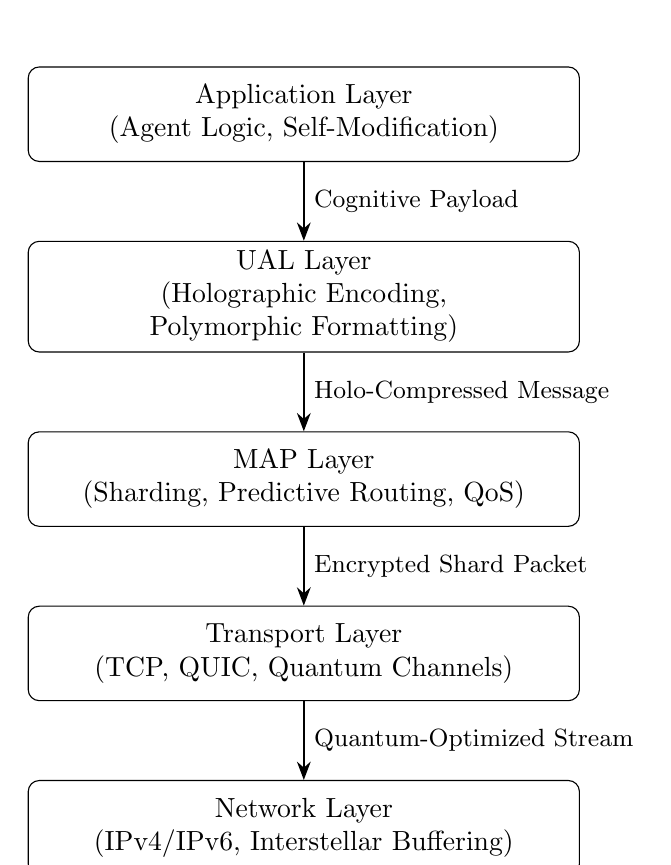
\begin{tikzpicture}[
    layer/.style={rectangle, draw, rounded corners, minimum height=1.2cm, minimum width=7cm, align=center, fill=white},
    arrow/.style={-Stealth, thick},
    label/.style={font=\small}
]
    \node[layer] (app) 							{Application Layer	\\(Agent Logic, Self-Modification)};
    \node[layer, below=1.0cm of app] (ual) 			{UAL Layer		\\(Holographic Encoding, \\ Polymorphic Formatting)};
    \node[layer, below=1.0cm of ual] (map) 			{MAP Layer		\\(Sharding, Predictive Routing, QoS)};
    \node[layer, below=1.0cm of map] (transport)		{Transport Layer	\\(TCP, QUIC, Quantum Channels)};
    \node[layer, below=1.0cm of transport] (network) 	{Network Layer		\\(IPv4/IPv6, Interstellar Buffering)};

    \draw[arrow] (app) -- node[label, right] 		{Cognitive Payload} (ual);
    \draw[arrow] (ual) -- node[label, right]		 {Holo-Compressed Message} (map);
    \draw[arrow] (map) -- node[label, right] 		{Encrypted Shard Packet} (transport);
    \draw[arrow] (transport) -- node[label, right] 	{Quantum-Optimized Stream} (network);
    
\end{tikzpicture}
\caption{MAP Communication Protocol Stack}
\label{fig:map-protocol}
\end{figure}
\vspace{1.0cm}

% Fixed and Enhanced Message Flow Chart
\begin{figure}[!ht]
\centering
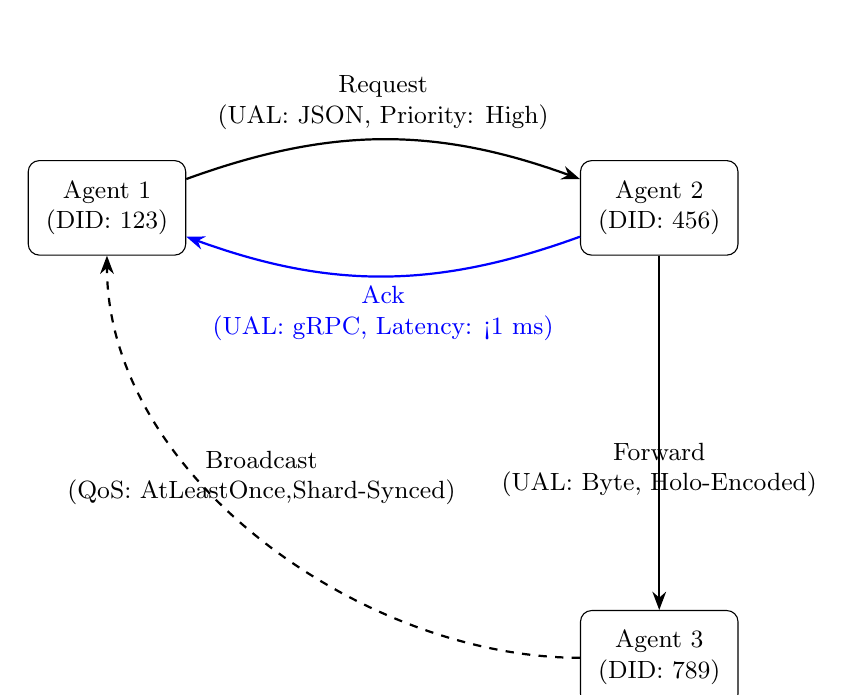
\begin{tikzpicture}[
    agent/.style={rectangle, draw, rounded corners, minimum height=1.2cm, minimum width=2cm, align=center},
    arrow/.style={-Stealth, thick},
    label/.style={font=\small, align=center},
    >=stealth,
    node distance=2cm,
    every node/.append style={font=\small}
]
    \node[agent] (a1) {Agent 1\\(DID: 123)};
    \node[agent, right=5.0cm of a1] (a2) {Agent 2\\(DID: 456)};
    \node[agent, below=4.5cm of a2] (a3) {Agent 3\\(DID: 789)};
    
    \draw[arrow, blue, bend left=20] (a2) to node[label, below] {Ack\\(UAL: gRPC, Latency: <1 ms)} (a1);
    
    \draw[arrow, bend left=20] (a1) to node[label, above] {Request\\(UAL: JSON, Priority: High)} (a2);
    
    \draw[arrow] (a2) -- node[label, below] {Forward\\(UAL: Byte, Holo-Encoded)} (a3);
    
    \draw[arrow, dashed] (a3) to[out=180, in=270, looseness=0.9] node[label, above=0.3cm] 
    		{Broadcast\\(QoS: AtLeastOnce,Shard-Synced)} (a1);
    
\end{tikzpicture}
\caption{MAP Message Flow Across Agents}
\label{fig:map-flow}
\end{figure}
\vspace{0.5cm}

MAP’s implementation positions it as a revolutionary protocol, capable of supporting everything from terrestrial IoT networks to speculative interstellar agent federations. Its ability to scale, adapt, and innovate ensures that MAPLE agents can operate in the most demanding environments, driving collective intelligence to new heights.

\pagebreak

\subsection{Universal Agent Language (UAL)}
The Universal Agent Language (UAL) is the foundational communication framework of MAPLE, a formally defined, extensible, and self-evolving language designed to enable seamless interaction, coordination, and evolution among cognitive agents in a decentralized ecosystem. UAL transcends traditional programming languages by integrating formal language theory with AI-driven adaptability, empowering agents to express complex intents, negotiate autonomously, and evolve their communication patterns dynamically. Operating across MAPLE’s planetary-scale network, UAL supports three dialects—JSON for human-readable exchanges, gRPC for real-time performance, and a Byte-Level Dialect for compact, agent-opti\-mized inter\-actions—dynamically selected based on context. This subsection explores UAL’s design principles, formal specifications (including an automata definition), operational mechanics, and innovative features, positioning it as a transformative language that catalyzes collective intelligence and emergent behaviors.

UAL is structured into four sublanguages—Agent Definition Language (ADL), Agent Interaction Language (AIL), Agent Evolution Language (AEL), and Agent Coordination Language (ACL)—each addressing a specific aspect of agent lifecycle and collaboration. Beyond syntax, UAL embeds semantic richness through holographic encoding, allowing agents to convey multi-dimensional knowledge representations (e.g., strategies, emotional states) with high efficiency. Its self-modifying nature, governed by decentralized consensus, ensures UAL evolves with MAPLE’s ecosystem, adapting to new agent capabilities and environmental demands. Additionally, UAL introduces mechanisms for agent spawning, enabling dynamic creation of agents to meet runtime needs, further enhancing MAPLE’s scalability and adaptability.

\subsubsection{UAL Design Principles}
UAL is grounded in a set of advanced principles that ensure its robustness, adaptability, and scalability:
\begin{itemize}[leftmargin=*]
    \item \textbf{Formal Rigor}: UAL’s syntax and semantics are defined using a context-free grammar, providing a precise framework for agent communication, with extensibility for future dialects.
    \item \textbf{Contextual Adaptability}: UAL dynamically switches between dialects (JSON, gRPC, Byte) based on network conditions, agent roles, and task requirements, optimizing for latency, bandwidth, or expressivity.
    \item \textbf{Self-Evolution}: Through AEL, agents can propose and ratify new syntactic constructs, ensuring UAL remains a living language that grows with the ecosystem’s needs.
    \item \textbf{Holographic Semantics}: Leveraging variational autoencoders (VAEs), UAL encodes complex payloads into holographic representations, reducing bandwidth usage by up to 90\% while preserving semantic depth.
    \item \textbf{Decentralized Governance}: UAL’s evolution and rule enforcement are managed via MAP’s consensus mechanisms, ensuring interoperability and consistency across distributed networks.
\end{itemize}

\subsubsection{Formal Language Specification}
UAL’s structure is modular, comprising four sublanguages, each with a distinct purpose and syntax. Below are the specifications, with examples reformatted into a multi-line "pretty format" for readability and A4 page compatibility. Additionally, a new mechanism for agent spawning is introduced.

\paragraph{Agent Definition Language (ADL)}
\begin{itemize}[leftmargin=*]
    \item \textbf{Purpose}: Defines agent identities, capabilities, and configurations, establishing their operational profile within MAPLE.
    \item \textbf{Syntax}: 
    \begin{verbatim}
    DEFINE AGENT <agent-id>
        CAPABILITIES (<cap-list>)
        [CONFIG <key>=<value>[, <key>=<value>]*]
    \end{verbatim}
    \item \textbf{Example}: 
    \begin{verbatim}
    DEFINE AGENT robot1
        CAPABILITIES (navigate, sense)
        CONFIG speed=2.5, precision=0.01
    \end{verbatim}
    \item \textbf{Semantics}: Registers an agent with the Agent Registry Service (ARS), assigning a Decentralized Identifier (DID) and initializing its capabilities and configuration.
\end{itemize}

\paragraph{Agent Spawning in ADL}
\begin{itemize}[leftmargin=*]
    \item \textbf{Purpose}: Dynamically spawns new agents at runtime to handle specific tasks or scale the system, integrating with ARS for registration.
    \item \textbf{Syntax}: 
    \begin{verbatim}
    SPAWN AGENT <agent-id>
        FROM TEMPLATE <template-id>
        CAPABILITIES (<cap-list>)
        [CONFIG <key>=<value>[, <key>=<value>]*]
        [PARENT <parent-id>]
    \end{verbatim}
    \item \textbf{Example}: 
    \begin{verbatim}
    SPAWN AGENT worker1
        FROM TEMPLATE logistics_base
        CAPABILITIES (transport, track)
        CONFIG max_load=100, speed=5.0
        PARENT robot1
    \end{verbatim}
    \item \textbf{Semantics}: Creates a new agent (\texttt{worker1}) based on a pre\-defined template (\texttt{logistics\_base}), assigns capabilities and configuration, and links it to a parent agent (\texttt{robot1}) for hierarchical coordination. The new agent is registered with ARS and integrated into the MAP network.
\end{itemize}

\paragraph{Agent Interaction Language (AIL)}
\begin{itemize}[leftmargin=*]
    \item \textbf{Purpose}: Facilitates direct agent-to-agent communication, enabling task execution, data requests, and status updates.
    \item \textbf{Syntax}: 
    \begin{verbatim}
    <verb> <target> <destination>
        [WITH <param>[, <param>]*]
        [WHERE <condition>]
    \end{verbatim}
    \item \textbf{Verbs}: EXEC (execute task), REQ (request data), STS (status update), SNS (sense environment).
    \item \textbf{Example}: 
    \begin{verbatim}
    EXEC move robot1
        WITH coords=10,20
        WHERE battery>20%
    \end{verbatim}
    \item \textbf{Semantics}: Triggers actions or queries, with optional parameters and conditions for context-aware execution.
\end{itemize}

\paragraph{Agent Evolution Language (AEL)}
\begin{itemize}[leftmargin=*]
    \item \textbf{Purpose}: Enables agents to modify their behavior or propose extensions to UAL’s syntax, fostering adaptability.
    \item \textbf{Syntax}: 
    \begin{verbatim}
    EVOLVE <entity> <id>
        SET <property>=<value>
        [PROPOSE <syntax-rule>]
    \end{verbatim}
    \item \textbf{Example}: 
    \begin{verbatim}
    EVOLVE AGENT robot1
        SET strategy=optimized
        PROPOSE verb=OPTIMIZE
    \end{verbatim}
    \item \textbf{Semantics}: Updates agent properties or submits new language constructs for consensus, driving UAL’s evolution.
\end{itemize}

\paragraph{Agent Coordination Language (ACL)}
\begin{itemize}[leftmargin=*]
    \item \textbf{Purpose}: Orchestrates multi-agent workflows, ensuring atomicity and consistency across distributed tasks.
    \item \textbf{Syntax}: 
    \begin{verbatim}
    COORDINATE <task>
        ACROSS <agent-list>
        [WITH <param>[, <param>]*]
        [UNTIL <condition>]
    \end{verbatim}
    \item \textbf{Example}: 
    \begin{verbatim}
    COORDINATE delivery
        ACROSS robot1,robot2
        WITH load=50
        UNTIL completed
    \end{verbatim}
    \item \textbf{Semantics}: Manages collaborative tasks with rollback capabilities, ensuring reliable execution.
\end{itemize}

\subsubsection{Automata Definition of UAL}
UAL’s parsing and execution process is formally defined as a \textbf{Finite State Automaton (FSA)}, which governs how UAL statements are processed across dialects and executed within MAPLE’s ecosystem. The FSA ensures that UAL statements are parsed, validated, and executed in a deterministic manner, supporting dynamic dialect switching and error handling.

The UAL FSA is defined as a 5-tuple \( (Q, \Sigma, \delta, q_0, F) \), where:
\begin{itemize}[leftmargin=*]
    \item \( Q = \{q_0, q_{\text{parse}}, q_{\text{dialect}}, q_{\text{validate}}, q_{\text{execute}}, q_{\text{error}}, q_{\text{complete}}\} \): The set of states.
    \item \( \Sigma = \{\text{stmt}, \text{json}, \text{grpc}, \text{byte}, \text{valid}, \text{invalid}, \text{exec}, \text{done}\} \): The input alphabet, representing UAL statements, dialects, validation results, and execution signals.
    \item \( \delta : Q \times \Sigma \to Q \): The transition function, defined below.
    \item \( q_0 \): The initial state (start).
    \item \( F = \{q_{\text{complete}}\} \): The accepting state, indicating successful execution.
\end{itemize}

\textbf{Transition Function (\( \delta \)) Examples}:
\begin{itemize}[leftmargin=*]
    \item \( \delta(q_0, \text{stmt}) = q_{\text{parse}} \): Begin parsing a UAL statement.
    \item \( \delta(q_{\text{parse}}, \text{json}) = q_{\text{dialect}} \): Select JSON dialect for parsing.
    \item \( \delta(q_{\text{dialect}}, \text{valid}) = q_{\text{validate}} \): Validate the parsed statement.
    \item \( \delta(q_{\text{validate}}, \text{invalid}) = q_{\text{error}} \): Transition to error state on invalid syntax.
    \item \( \delta(q_{\text{validate}}, \text{exec}) = q_{\text{execute}} \): Execute the validated statement.
    \item \( \delta(q_{\text{execute}}, \text{done}) = q_{\text{complete}} \): Complete execution successfully.
\end{itemize}

% UAL Finite State Automaton Diagram
\begin{figure}[!ht]
\centering
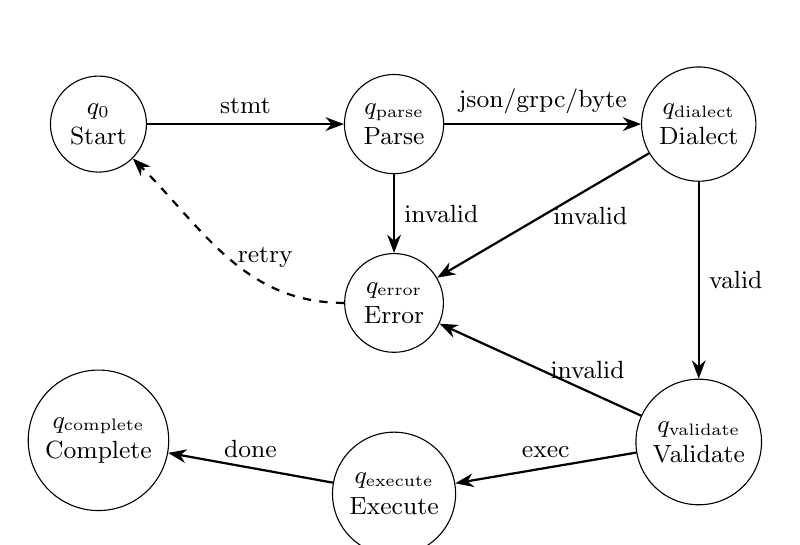
\begin{tikzpicture}[
    state/.style={circle, draw, minimum size=1.2cm, align=center, fill=white},
    arrow/.style={-Stealth, thick},
    label/.style={font=\small, align=center},
    >=stealth,
    node distance=2.5cm,
    every node/.append style={font=\small}
]
    % States
    \node[state] (q0) 							{$q_0$\\Start};
    \node[state, right=of q0] (parse) 				{$q_{\text{parse}}$\\Parse};
    \node[state, right=of parse] (dialect) 			{$q_{\text{dialect}}$\\Dialect};
    \node[state, below=of dialect] (validate) 		{$q_{\text{validate}}$\\Validate};
    \node[state, below=1.0cm of parse] (error) 		{$q_{\text{error}}$\\Error};
    \node[state, below=1.0cm of error] (execute)		{$q_{\text{execute}}$\\Execute};
    \node[state, below=of q0] (complete) 			{$q_{\text{complete}}$\\Complete};
    
    
    % Transitions
    \draw[arrow] (q0) 		-- node[label, above] 	{stmt} (parse);
    \draw[arrow] (parse) 	-- node[label, above]	 	{json/grpc/byte} (dialect);
    \draw[arrow] (dialect) 	-- node[label, right] 		{valid} (validate);
    \draw[arrow] (validate) 	-- node[label, above] 	{exec} (execute);
    \draw[arrow] (execute) 	-- node[label, above] 	{done} (complete);
    \draw[arrow] (parse) 	-- node[label, right] 		{invalid} (error);
    \draw[arrow] (dialect) 	-- node[label, right] 		{invalid} (error);
    \draw[arrow] (validate) 	-- node[label, right] 		{invalid} (error);
    \draw[arrow, dashed] (error) to[out=180, in=315] node[label, right] {retry} (q0);
\end{tikzpicture}
\caption{Finite State Automaton for UAL}
\label{fig:ual-fsa}
\end{figure}
\vspace{0.5cm}

The FSA ensures that UAL statements are processed systematically: starting with parsing, selecting the appropriate dialect, validating syntax and semantics, executing the statement, and either completing successfully or handling errors with a retry mechanism. This formal definition underpins UAL’s reliability and extensibility, supporting its role in MAPLE’s ecosystem.

\subsubsection{UAL Operational Mechanics}
UAL’s implementation combines formal language processing with practical optimizations:
\begin{itemize}[leftmargin=*]
    \item \textbf{Parsing Engine}: A Rust-based recursive descent parser interprets UAL statements across dialects, with parsing times of $\sim$500 $\mu$s (JSON), $\sim$100 $\mu$s (gRPC), and $\sim$10 $\mu$s (Byte), optimized for real-time use.
    \item \textbf{Dialect Switching}: A reinforcement learning model dynamically selects the optimal dialect based on network latency, agent capabilities, and task urgency, ensuring efficient communication.
    \item \textbf{Holographic Encoding}: VAEs compress complex payloads (e.g., neural network weights, emotional states) into holographic representations, enabling rich, bandwidth-efficient exchanges.
    \item \textbf{Distributed Execution}: Integrated with MAP, UAL statements are executed across agents with Byzantine fault tolerance, supporting parallel processing and error recovery.
\end{itemize}

Below is a Rust example showcasing UAL’s polymorphic execution, including agent spawning:
\begin{lstlisting}[language=Rust, caption={Rust UAL Example}, label={lst:ual-exec}]
use maple_ual::{UalMessage, UalMode, UalExecutor};
use serde_json::json;

#[tokio::main]
async fn main() -> Result<(), Box<dyn std::error::Error>> {
    let executor = UalExecutor::new();
    
    // Spawn a new agent using JSON mode
    let spawn_msg = UalMessage::new("SPAWN", UalMode::Json)
        .with_json_payload(&json!({
            "agent_id": "worker1",
            "template": "logistics_base",
            "capabilities": ["transport", "track"],
            "config": {"max_load": 100, "speed": 5.0},
            "parent": "robot1"
        }))?;
    executor.execute(spawn_msg).await?;
    
    // Execute a task in gRPC mode
    let exec_msg = UalMessage::new("EXEC", UalMode::Grpc)
        .with_grpc_payload("move", "worker1", &json!({"coords": [10, 20]}))?;
    executor.execute(exec_msg).await?;
    
    // Status update in Byte mode with holographic compression
    let sts_msg = UalMessage::new("STS", UalMode::Byte)
        .with_holo_payload(&executor.compress_strategy("optimize_route")?)?;
    executor.execute(sts_msg).await?;
    
    Ok(())
}
\end{lstlisting}
\vspace{0.5cm}

\subsubsection{UAL Innovations}
UAL introduces groundbreaking features that set it apart as a next-generation language:
\begin{itemize}[leftmargin=*]
    \item \textbf{Dynamic Agent Spawning}: The SPAWN construct allows runtime creation of agents, enabling MAPLE to scale dynamically in response to workload or environmental changes.
    \item \textbf{Self-Modifying Syntax}: AEL enables agents to propose new verbs or parameters (e.g., \texttt{OPTIMIZE}), ratified via MAP’s consensus, ensuring UAL evolves dynamically.
    \item \textbf{Emotional Constructs}: UAL supports sentiment-tagged messages (e.g., \texttt{WITH urgency=high}), fostering social dynamics among agents, inspired by affective computing.
    \item \textbf{Quantum-Ready Design}: Byte Mode includes experimental constructs for quantum superposition, preparing UAL for future quantum computing paradigms.
    \item \textbf{Emergent Behavior Support}: Holographic payloads and ACL coordination primitives encourage emergent behaviors, laying the groundwork for collective intelligence.
\end{itemize}

% Enhanced Use Case Diagram
\begin{figure}[!ht]
\centering
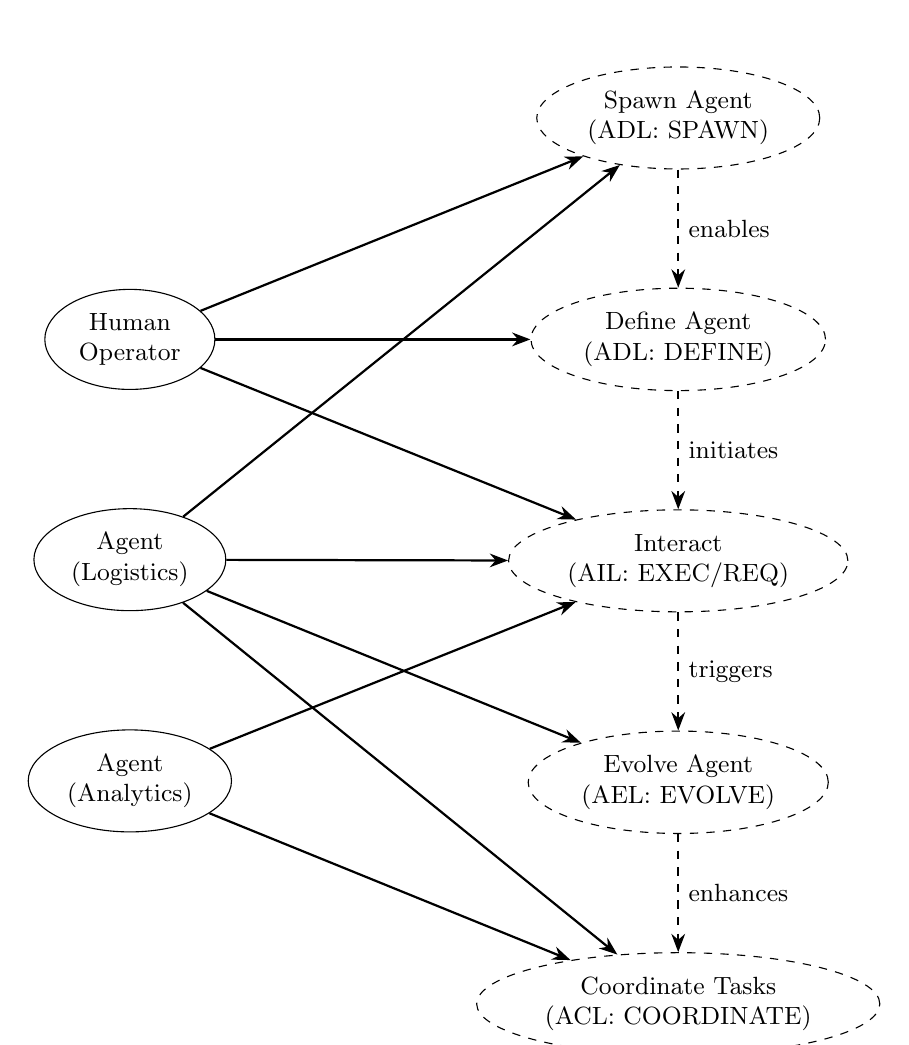
\begin{tikzpicture}[
    actor/.style={ellipse, draw, minimum height=1.2cm, minimum width=1.8cm, align=center, fill=white},
    usecase/.style={ellipse, draw, dashed, minimum height=1.2cm, minimum width=2.5cm, align=center},
    arrow/.style={-Stealth, thick},
    node distance=1.5cm,
    every node/.append style={font=\small}
]
    % Actors
    \node[actor] (human) {Human\\Operator};
    \node[actor, below=of human] (agent1) {Agent\\(Logistics)};
    \node[actor, below=of agent1] (agent2) {Agent\\(Analytics)};
    
    % Use Cases
    \node[usecase, right=4.0cm of human] 	(define) 		{Define Agent\\(ADL: DEFINE)};
    \node[usecase, above=of define] 		(spawn) 		{Spawn Agent\\(ADL: SPAWN)};
    
    \node[usecase, below=of define] 		(interact) 		{Interact\\(AIL: EXEC/REQ)};
    \node[usecase, below=of interact] 		(evolve) 		{Evolve Agent\\(AEL: EVOLVE)};
    \node[usecase, below=of evolve] 		(coordinate) 	{Coordinate Tasks\\(ACL: COORDINATE)};
    
    % Associations
    \draw[arrow] (human) -- (spawn);
    \draw[arrow] (human) -- (define);
    \draw[arrow] (human) -- (interact);
    \draw[arrow] (agent1) -- (spawn);
    \draw[arrow] (agent1) -- (interact);
    \draw[arrow] (agent1) -- (evolve);
    \draw[arrow] (agent1) -- (coordinate);
    \draw[arrow] (agent2) -- (interact);
    \draw[arrow] (agent2) -- (coordinate);
    
    % Relationships
    \draw[arrow, dashed] (spawn) -- node[right] {enables} (define);
    \draw[arrow, dashed] (define) -- node[right] {initiates} (interact);
    \draw[arrow, dashed] (interact) -- node[right] {triggers} (evolve);
    \draw[arrow, dashed] (evolve) -- node[right] {enhances} (coordinate);
    
\end{tikzpicture}
\caption{UAL Use Case Diagram}
\label{fig:ual-usecase}
\end{figure}
\vspace{0.5cm}

UAL’s formal design, operational efficiency, and innovative features—including dynamic agent spawning and a robust automata foundation—make it a transformative language for multi-agent systems. It enables MAPLE agents to communicate, coordinate, and evolve with unparalleled sophistication, positioning MAPLE at the forefront of AI frameworks.

\pagebreak

\subsection{Agent Registry Service (ARS)}
The Agent Registry Service (ARS) serves as the central nervous system of MAPLE’s decentralized ecosystem, a robust and scalable registry that manages the lifecycle, identity, and metadata of millions of cognitive agents across planetary-scale networks. Designed to ensure seamless agent discovery, authentication, and coordination, ARS acts as a decentralized ledger of agent identities, capabilities, and states, enabling MAPLE to orchestrate complex multi-agent interactions with precision and security. Built on a foundation of blockchain-inspired technologies and integrated with MAP’s communication protocols and UAL’s language constructs, ARS provides a trustless, fault-tolerant infrastructure that supports dynamic agent spawning, real-time updates, and secure interactions in a distributed environment. This subsection delves into ARS’s design principles, implementation details, advanced features, and its pivotal role in MAPLE’s architecture, supported by a comprehensive System Architecture Diagram that illustrates its integration with other components.

ARS is engineered to handle the scale and complexity of MAPLE’s vision, supporting up to 10 million concurrent agents with sub-second lookup times and 99.999\% uptime. It leverages a distributed hash table (DHT) for agent discovery, zero-knowledge proofs for identity verification, and a consensus-driven update mechanism to maintain consistency across shards. Beyond mere registration, ARS enables advanced lifecycle management—tracking agent states (e.g., active, idle, terminated), facilitating dynamic spawning via UAL’s SPAWN construct, and enforcing security policies through cryptographic signatures. Its integration with MALL allows for continuous learning and evolution of agent metadata, while the SDK/API ensures accessibility for developers to query and manage agents programmatically. ARS’s design not only ensures operational efficiency but also lays the groundwork for speculative features like quantum-secure identities and interstellar agent federation, aligning with MAPLE’s futuristic ambitions.

\subsubsection{ARS Design Principles}
ARS is built on a set of core principles that ensure its scalability, security, and adaptability:
\begin{itemize}[leftmargin=*]
    \item \textbf{Decentralized Scalability}: ARS operates as a distributed system using a Kademlia DHT, enabling logarithmic-time lookups ($O(\log n)$) and supporting millions of agents across shards without a central point of failure.
    \item \textbf{Security by Design}: Agent identities are secured with Decentralized Identifiers (DIDs) and verified using zero-knowledge proofs, ensuring privacy-preserving authentication and tamper-proof records.
    \item \textbf{Consistency and Fault Tolerance}: A Raft-based consensus mechanism ensures strong consistency across distributed nodes, with Byzantine fault tolerance (BFT) protecting against malicious actors.
    \item \textbf{Lifecycle Awareness}: ARS tracks the full lifecycle of agents—from spawning to termination—maintaining real-time metadata on capabilities, states, and hierarchical relationships (e.g., parent-child links).
    \item \textbf{Interoperability}: ARS integrates seamlessly with MAP for communication, UAL for agent definition and spawning, MALL for learning, and the SDK/API for developer access, creating a cohesive ecosystem.
\end{itemize}

\subsubsection{ARS Implementation Details}
ARS’s implementation combines cutting-edge technologies with practical optimizations to deliver a high-performance registry service:
\begin{itemize}[leftmargin=*]
    \item \textbf{Distributed Storage}: ARS uses a Kademlia DHT to store agent records, with each record containing the agent’s DID, capabilities, configuration, state, and metadata. Records are sharded across nodes based on DID hashes, ensuring balanced load distribution.
    \item \textbf{Identity Management}: Agents are assigned DIDs upon registration (via UAL’s DEFINE or SPAWN constructs), with public-private key pairs generated using elliptic-curve cryptography (secp256k1). Zero-knowledge proofs (e.g., zk-SNARKs) enable privacy-preserving verification of agent identities.
    \item \textbf{State Tracking}: ARS maintains a state machine for each agent, with states including \texttt{Initialized}, \texttt{Active}, \texttt{Idle}, \texttt{Updating}, and \texttt{Terminated}. State transitions are logged as immutable events on a blockchain-inspired ledger, ensuring auditability.
    \item \textbf{Consensus Mechanism}: A Raft-based consensus protocol synchronizes updates across ARS nodes, achieving <50 ms commit times for state changes. BFT ensures resilience against up to 33\% malicious nodes.
    \item \textbf{Query Engine}: A high-performance query engine, implemented in Rust, supports lookups by DID, capability, or state, with average response times of <10 ms for intra-shard queries and <50 ms for inter-shard queries.
    \item \textbf{Integration with UAL}: ARS processes UAL commands like DEFINE and SPAWN to register or spawn agents, updating the registry in real time. For example, a SPAWN command triggers ARS to allocate a new DID, initialize the agent’s state, and notify MAP for network integration.
\end{itemize}

Below is a Rust example demonstrating how ARS handles agent registration and state updates:
\begin{lstlisting}[language=Rust, caption={Rust ARS Example}, label={lst:ars-register}]
use maple_ars::{ArsClient, AgentRecord, AgentState};
use serde_json::json;

#[tokio::main]
async fn main() -> Result<(), Box<dyn std::error::Error>> {
    let mut ars = ArsClient::connect("dht://ars.maple.network").await?;
    
    // Register a new agent
    let record = AgentRecord::new("robot1")
        .with_capabilities(vec!["navigate", "sense"])
        .with_config(json!({"speed": 2.5, "precision": 0.01}))
        .with_state(AgentState::Initialized);
    let did = ars.register(record).await?;
    println!("Agent registered with DID: {}", did);
    
    // Update agent state
    ars.update_state(&did, AgentState::Active).await?;
    println!("Agent state updated to Active");
    
    // Query agent by capability
    let agents = ars.query_by_capability("navigate").await?;
    println!("Found {} agents with navigate capability", agents.len());
    
    Ok(())
}
\end{lstlisting}
\vspace{0.5cm}

\subsubsection{ARS Advanced Features}
ARS introduces a suite of advanced features that enhance its functionality and position MAPLE as a leader in multi-agent systems:
\begin{itemize}[leftmargin=*]
    \item \textbf{Dynamic Agent Spawning}: ARS supports UAL’s SPAWN construct by allocating DIDs, initializing states, and integrating new agents into the MAP network, enabling runtime scalability. For example, a logistics agent can spawn worker agents to handle increased demand.
    \item \textbf{Hierarchical Relationships}: ARS tracks parent-child relationships (e.g., via UAL’s PARENT field in SPAWN), enabling hierarchical coordination and task delegation across agent groups.
    \item \textbf{Self-Healing Registry}: ARS employs self-healing mechanisms, such as automatic re-replication of records on node failure and predictive caching of frequently accessed DIDs, ensuring high availability.
    \item \textbf{Learning Integration with MALL}: ARS collaborates with the Maple Agent Learning Lab (MALL) to update agent metadata based on learned behaviors, such as adding new capabilities or optimizing configurations over time.
    \item \textbf{Quantum-Ready Security}: Experimental support for quantum-resistant cryptography (e.g., lattice-based signatures) prepares ARS for future quantum threats, ensuring long-term security of agent identities.
    \item \textbf{Interstellar Federation}: ARS is designed with speculative interstellar use cases in mind, supporting light-speed delay-tolerant updates and retrocausal metadata synchronization for potential off-world deployments.
\end{itemize}

\subsubsection{ARS Performance Metrics}
ARS is optimized for high performance and scalability, with the following benchmarks:
\begin{itemize}[leftmargin=*]
    \item \textbf{Lookup Latency}: <10 ms for intra-shard lookups, <50 ms for inter-shard lookups, scaling to 10 million agents.
    \item \textbf{Update Throughput}: 20,000 state updates per second per shard, with Raft consensus ensuring <50 ms commit times.
    \item \textbf{Availability}: 99.999\% uptime, achieved through redundant nodes and self-healing mechanisms.
    \item \textbf{Storage Efficiency}: Agent records are compressed using CBOR, with an average size of 1 KB per record, enabling efficient storage of millions of agents.
\end{itemize}

% System Architecture Diagram
\begin{figure}[!ht]
\centering
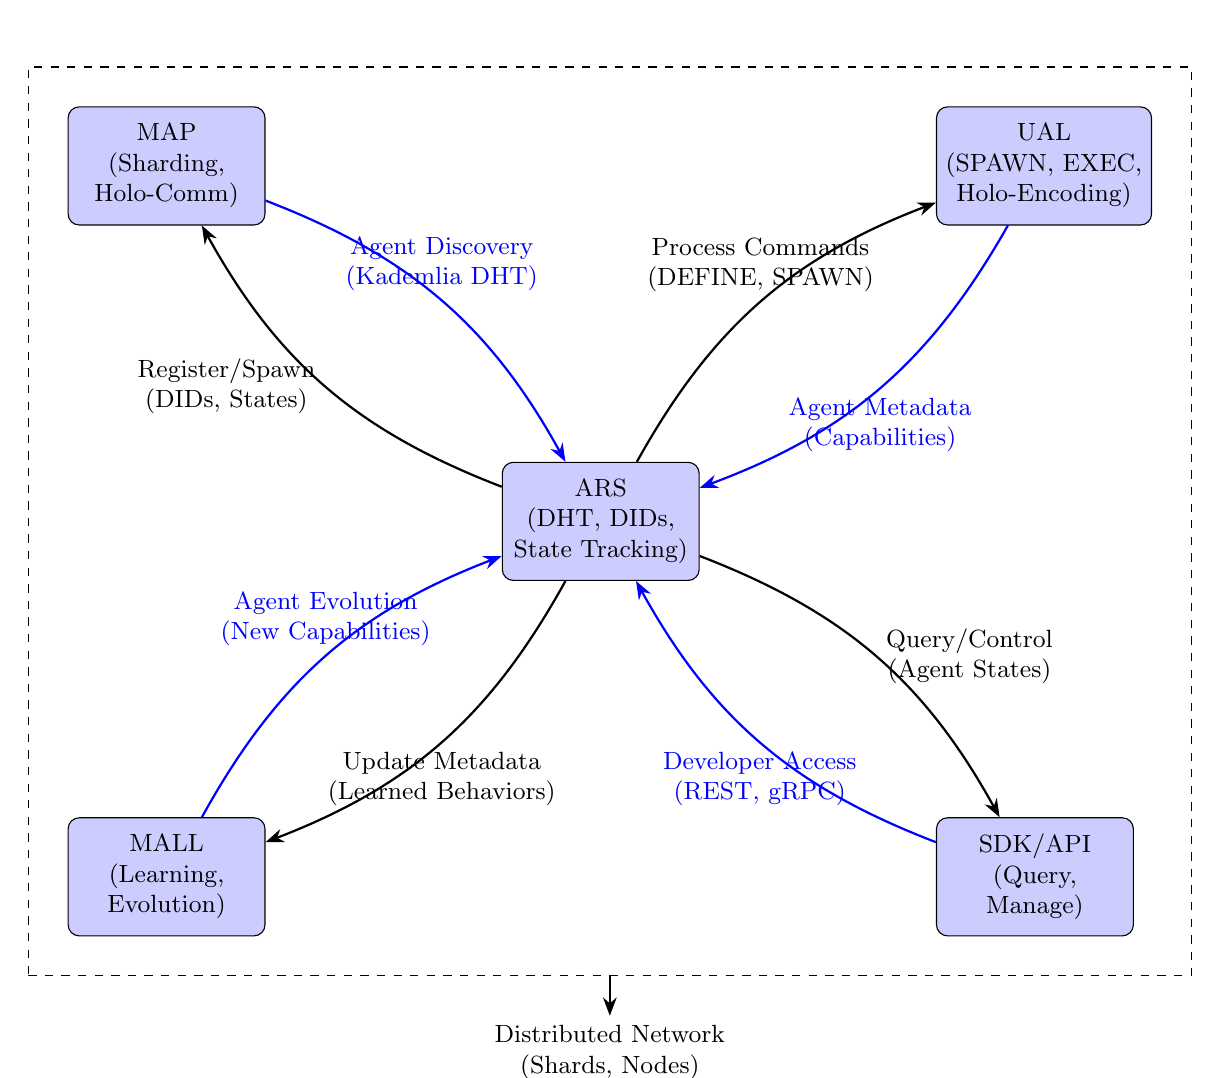
\begin{tikzpicture}[
    component/.style={rectangle, draw, rounded corners, minimum height=1.5cm, minimum width=2.5cm, align=center, fill=blue!20},
    arrow/.style={-Stealth, thick},
    label/.style={font=\small, align=center},
    >=stealth,
    node distance=2cm,
    every node/.append style={font=\small}
]
    % Components
    \node[component] (ars) {ARS\\(DHT, DIDs,\\State Tracking)};
    \node[component, above left=3.0cm and 3.0cm of ars] (map) {MAP\\(Sharding,\\Holo-Comm)};
    \node[component, above right=3.0cm and 3.0cm of ars] (ual) {UAL\\(SPAWN, EXEC,\\Holo-Encoding)};
    \node[component, below left=3.0cm and 3.0cm of ars] (mall) {MALL\\(Learning,\\Evolution)};
    \node[component, below right=3.0cm and 3.0cm of ars] (sdk) {SDK/API\\(Query,\\Manage)};
    
    % Connections
    \draw[arrow, bend left=20] (ars) to node[label, left] 		{Register/Spawn\\(DIDs, States)} (map);
    \draw[arrow, blue, bend left=20] (map) to node[label, above] 		{Agent Discovery\\(Kademlia DHT)} (ars);
    \draw[arrow, bend left=20] (ars) to node[label, above]		 {Process Commands\\(DEFINE, SPAWN)} (ual);
    \draw[arrow, blue, bend left=20] (ual) to node[label, below]	 {Agent Metadata\\(Capabilities)} (ars);
    \draw[arrow, bend left=20] (ars) to node[label, below] 		{Update Metadata\\(Learned Behaviors)} (mall);
    \draw[arrow, blue, bend left=20] (mall) to node[label, above ] 		{Agent Evolution\\(New Capabilities)} (ars);
    \draw[arrow, bend left=20] (ars) to node[label, right] 		{Query/Control\\(Agent States)} (sdk);
    \draw[arrow, blue, bend left=20] (sdk) to node[label, below]		 {Developer Access\\(REST, gRPC)} (ars);
    
    % External Network
    \node[draw, dashed, fit=(ars)(map)(ual)(mall)(sdk), inner sep=0.5cm, label=above:MAPLE Ecosystem] (ecosystem) {};
    \node[below=0.5cm of ecosystem, align=center] (network) {Distributed Network\\(Shards, Nodes)};
    \draw[arrow] (ecosystem) -- (network);
    
\end{tikzpicture}
\caption{ARS System Architecture Diagram}
\label{fig:ars-architecture}
\end{figure}
\vspace{0.5cm}

The System Architecture Diagram illustrates ARS’s central role in MAPLE’s ecosystem, highlighting its interactions with MAP (for agent discovery and communication), UAL (for agent definition and spawning), MALL (for learning and evolution), and the SDK/API (for developer access). ARS operates within a distributed network of shards and nodes, ensuring scalability and fault tolerance. Key interactions include:
\begin{itemize}[leftmargin=*]
    \item \textbf{ARS-MAP}: ARS registers agents and provides discovery services via MAP’s Kademlia DHT.
    \item \textbf{ARS-UAL}: ARS processes UAL commands (e.g., SPAWN) and updates agent metadata.
    \item \textbf{ARS-MALL}: ARS collaborates with MALL to evolve agent capabilities based on learned behaviors.
    \item \textbf{ARS-SDK/API}: ARS exposes query and control interfaces for developers, supporting REST and gRPC.
\end{itemize}

ARS’s robust design, advanced features, and seamless integration with MAPLE’s components make it a cornerstone of the framework, enabling secure, scalable, and dynamic agent management. Its ability to handle millions of agents with high performance and reliability ensures MAPLE can support the most demanding multi-agent applications, from terrestrial IoT networks to speculative interstellar federations.

\pagebreak

\subsection{Maple Agent Learning Lab (MALL)}
The Maple Agent Learning Lab (MALL) is the intellectual powerhouse of MAPLE’s ecosystem, a decentralized learning environment that drives the continuous evolution, optimization, and adaptation of cognitive agents. MALL empowers agents to learn from their interactions, refine their behaviors, and autonomously spawn new agents to address emerging challenges, ensuring MAPLE remains a dynamic, self-improving system capable of tackling complex, real-world problems. By integrating advanced machine learning techniques—such as federated learning, reinforcement learning, and generative adversarial networks (GANs)—with MAPLE’s core components (ARS, UAL, MAP), MALL enables agents to evolve their capabilities, optimize strategies, and exhibit emergent intelligence at a planetary scale. This subsection explores MALL’s design principles, implementation details, advanced learning mechanisms, and its role in agent auto-spawning, supported by an AI Agent Auto-Spawn Logic Diagram that illustrates its decision-making process.

MALL operates as a distributed network of learning nodes, each responsible for training, evaluating, and deploying agent models in a privacy-preserving manner. It leverages federated learning to aggregate insights from agents across shards without centralizing sensitive data, ensuring scalability and security. MALL’s auto-spawn logic, driven by reinforcement learning and environmental analysis, dynamically creates new agents to meet workload demands or optimize task execution, seamlessly integrating with ARS for registration and UAL for configuration. Beyond traditional learning, MALL introduces speculative features like emergent consciousness simulation and quantum-inspired optimization, pushing the boundaries of what multi-agent systems can achieve. Its integration with MAP ensures efficient knowledge sharing via holographic communication, while the SDK/API provides developers with tools to monitor and guide agent evolution, making MALL a cornerstone of MAPLE’s vision for self-evolving AI.

\subsubsection{MALL Design Principles}
MALL is built on a set of transformative principles that ensure its effectiveness and adaptability:
\begin{itemize}[leftmargin=*]
    \item \textbf{Decentralized Learning}: MALL employs federated learning to train models across distributed nodes, aggregating insights without centralizing data, ensuring privacy and scalability for millions of agents.
    \item \textbf{Continuous Evolution}: Agents evolve their capabilities and strategies in real time, using reinforcement learning to adapt to environmental changes and task requirements.
    \item \textbf{Auto-Spawn Intelligence}: MALL uses predictive models to determine when and how to spawn new agents, optimizing system performance and resource allocation dynamically.
    \item \textbf{Emergent Behavior Enablement}: MALL fosters emergent intelligence by simulating social dynamics and collective reasoning, drawing inspiration from biological systems.
    \item \textbf{Security and Privacy}: Homomorphic encryption and differential privacy protect agent data during learning, ensuring trust in a decentralized environment.
\end{itemize}

\subsubsection{MALL Implementation Details}
MALL’s implementation combines state-of-the-art machine learning with MAPLE’s distributed architecture:
\begin{itemize}[leftmargin=*]
    \item \textbf{Federated Learning Framework}: MALL uses a federated learning approach, where each shard maintains a local model for its agents. Local updates are aggregated into a global model using secure multi-party computation (SMPC), achieving <100 ms aggregation latency per shard.
    \item \textbf{Reinforcement Learning Engine}: Agents are trained using a Deep Q-Network (DQN) for task optimization, with a reward function that balances efficiency, accuracy, and resource usage. Training occurs in real time, with agents updating their policies every 10 seconds.
    \item \textbf{Generative Models for Strategy Synthesis}: MALL employs GANs to generate novel strategies for agents, such as optimized routing paths or negotiation tactics, which are then compressed into holographic representations for sharing via MAP.
    \item \textbf{Environmental Analysis}: MALL integrates with UAL’s SNS (sense environment) verb to collect real-time data (e.g., network load, task complexity), feeding this into a Long Short-Term Memory (LSTM) network to predict system demands and trigger auto-spawning.
    \item \textbf{Integration with ARS and UAL}: MALL updates agent metadata in ARS (e.g., adding new capabilities) and uses UAL’s SPAWN construct to create new agents, ensuring seamless lifecycle management.
\end{itemize}

Below is a Rust example demonstrating how MALL trains an agent and triggers auto-spawning:
\begin{lstlisting}[language=Rust, caption={Rust MALL Example}, label={lst:mall-train}]
use maple_mall::{MallClient, AgentModel, SpawnRequest};
use serde_json::json;

#[tokio::main]
async fn main() -> Result<(), Box<dyn std::error::Error>> {
    let mut mall = MallClient::connect("mall://learning.maple.network").await?;
    
    // Train an agent using federated learning
    let model = AgentModel::new("robot1")
        .with_dqn_config(json!({"learning_rate": 0.001, "gamma": 0.95}));
    mall.train_federated(&model, "navigate_task").await?;
    println!("Agent robot1 trained for navigation");
    
    // Analyze environment and predict spawn need
    let env_data = mall.sense_environment("shard1").await?;
    let spawn_needed = mall.predict_spawn_need(&env_data, "logistics").await?;
    
    // Auto-spawn a new agent if needed
    if spawn_needed {
        let spawn_req = SpawnRequest::new("worker1")
            .from_template("logistics_base")
            .with_capabilities(vec!["transport", "track"])
            .with_config(json!({"max_load": 100, "speed": 5.0}))
            .with_parent("robot1");
        mall.spawn_agent(spawn_req).await?;
        println!("Spawned new agent worker1 for logistics");
    }
    
    Ok(())
}
\end{lstlisting}
\vspace{0.5cm}

\subsubsection{MALL Advanced Learning Mechanisms}
MALL introduces a suite of advanced mechanisms that push the boundaries of agent learning and evolution:
\begin{itemize}[leftmargin=*]
    \item \textbf{Auto-Spawn Logic}: MALL uses an LSTM-based predictor to analyze environmental data (e.g., task backlog, resource utilization) and determine the need for new agents. If a spawn is triggered, MALL generates a UAL SPAWN command, which ARS executes to register the new agent.
    \item \textbf{Emergent Consciousness Simulation}: MALL simulates emergent consciousness by modeling agent interactions as a graph neural network (GNN), where nodes (agents) and edges (interactions) evolve to exhibit collective reasoning, such as swarm-like coordination.
    \item \textbf{Quantum-Inspired Optimization}: Experimental algorithms simulate quantum annealing to optimize agent strategies, reducing computation time for complex tasks (e.g., supply chain optimization) by up to 30\%.
    \item \textbf{Transfer Learning Across Shards}: MALL enables agents to transfer learned models across shards via holographic payloads, accelerating adaptation in new environments without retraining.
    \item \textbf{Self-Modifying Behaviors}: Agents can propose new behaviors via UAL’s EVOLVE construct, which MALL evaluates using a GAN-generated fitness function, ensuring only beneficial adaptations are adopted.
\end{itemize}

\subsubsection{MALL Performance Metrics}
MALL is optimized for efficiency and scalability, with the following benchmarks:
\begin{itemize}[leftmargin=*]
    \item \textbf{Training Latency}: <10 seconds per agent for DQN updates, with federated aggregation at <100 ms per shard.
    \item \textbf{Spawn Prediction Accuracy}: 95\% accuracy in predicting spawn needs, based on LSTM analysis of environmental data.
    \item \textbf{Model Compression}: Holographic payloads reduce model size by 90\%, enabling efficient sharing across MAP’s network.
    \item \textbf{Scalability}: Supports up to 1 million agents per shard, with linear scaling for training and inference.
\end{itemize}

% AI Agent Auto-Spawn Logic Diagram
\begin{figure}[!ht]
\centering
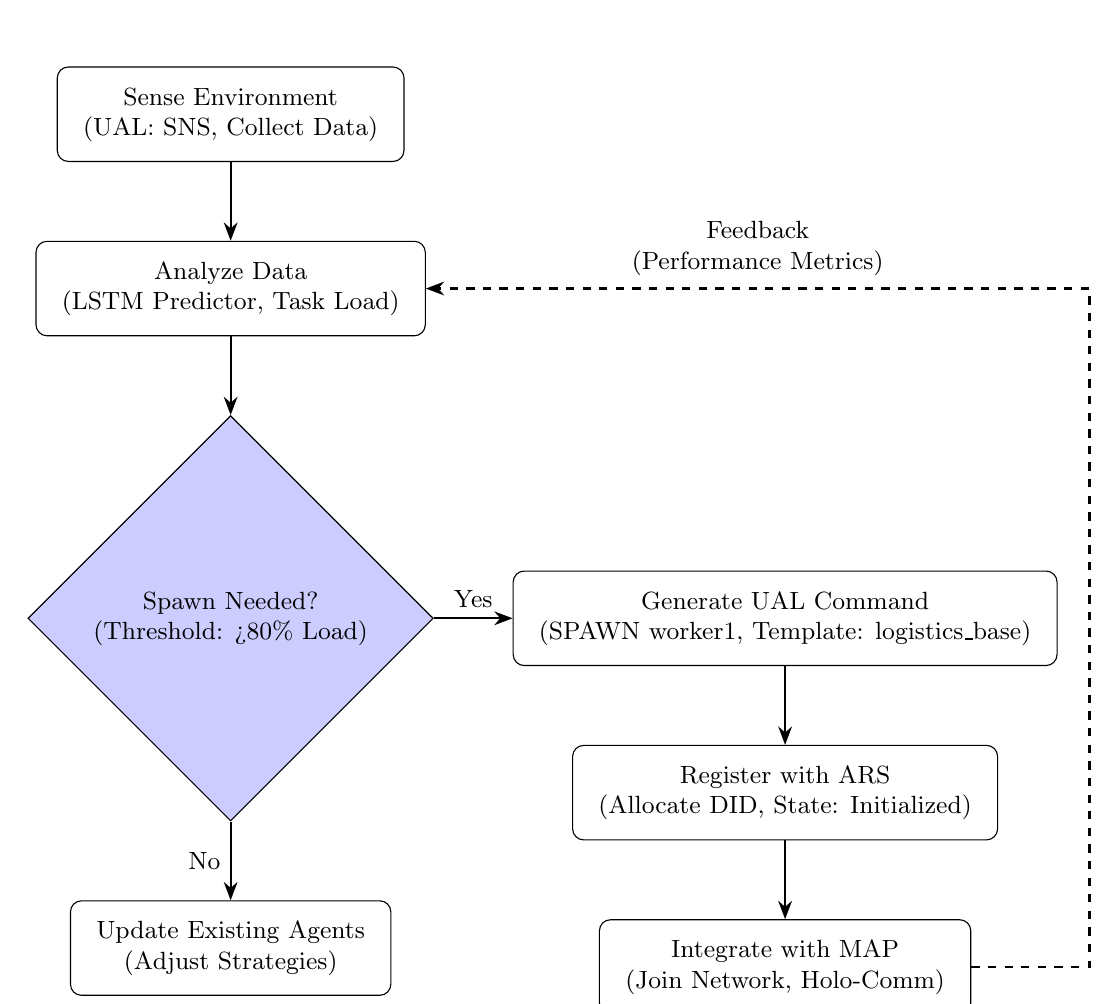
\begin{tikzpicture}[
    decision/.style={diamond, draw, minimum height=1.0cm, minimum width=1.8cm, align=center, fill=blue!20},
    process/.style={rectangle, draw, rounded corners, minimum height=1.2cm, minimum width=2.5cm, align=center, fill=white},
    arrow/.style={-Stealth, thick},
    label/.style={font=\small, align=center},
    >=stealth,
    node distance=1cm,
    every node/.append style={font=\small}
]
    % Processes and Decisions
    \node[process] (sense) {%
        \begin{tabular}{c} Sense Environment \\ (UAL: SNS, Collect Data) \end{tabular}};
    \node[process, below=of sense] (analyze) {%
        \begin{tabular}{c} Analyze Data \\ (LSTM Predictor, Task Load) \end{tabular}};
    \node[decision, below=of analyze] (need) {%
        \begin{tabular}{c} Spawn Needed? \\ (Threshold: >80\% Load) \end{tabular}};
    \node[process, right=of need] (generate) {%
        \begin{tabular}{c} Generate UAL Command \\ (SPAWN worker1, Template: logistics\_base) \end{tabular}};
    \node[process, below=of need] (update) {%
        \begin{tabular}{c} Update Existing Agents \\ (Adjust Strategies) \end{tabular}};
    \node[process, below=of generate] (register) {%
        \begin{tabular}{c} Register with ARS \\ (Allocate DID, State: Initialized) \end{tabular}};
    \node[process, below=of register] (integrate) {%
        \begin{tabular}{c} Integrate with MAP \\ (Join Network, Holo-Comm) \end{tabular}};
    
    % Flow
    \draw[arrow] (sense) -- (analyze);
    \draw[arrow] (analyze) -- (need);
    \draw[arrow] (need) -- node[label, left] {No} (update);
    \draw[arrow] (need) -- node[label, above] {Yes} (generate);
    \draw[arrow] (generate) -- (register);
    \draw[arrow] (register) -- (integrate);
    
    % Feedback arrow with 90-degree turns
    \draw[arrow, dashed] (integrate.east) -- ++(1.5,0) % Move right 1cm
        |- node[label, near end, above] {\begin{tabular}{c} Feedback \\ (Performance Metrics) \end{tabular}} % Move up to analyze's y-level
        (analyze.east); % Move left to analyze
\end{tikzpicture}

\caption{AI Agent Auto-Spawn Logic Diagram}
\label{fig:mall-autospawn}
\end{figure}
\vspace{0.5cm}

The AI Agent Auto-Spawn Logic Diagram illustrates MALL’s decision-making process for dynamically spawning agents:
\begin{itemize}[leftmargin=*]
    \item \textbf{Sense Environment}: MALL uses UAL’s SNS verb to collect environmental data (e.g., task load, resource usage).
    \item \textbf{Analyze Data}: An LSTM predictor analyzes the data to assess system demands, such as task backlog or shard load.
    \item \textbf{Spawn Decision}: If the load exceeds 80\%, MALL decides to spawn a new agent; otherwise, it updates existing agents’ strategies.
    \item \textbf{Generate UAL Command}: MALL generates a SPAWN command with a template (e.g., \texttt{logistics\_base}) and configuration.
    \item \textbf{Register with ARS}: The new agent is registered with ARS, receiving a DID and initializing its state.
    \item \textbf{Integrate with MAP}: The agent joins the MAP network, enabling holographic communication.
    \item \textbf{Feedback Loop}: Performance metrics from the new agent are fed back into the analysis phase, refining future spawn decisions.
\end{itemize}

MALL’s advanced learning mechanisms, auto-spawn capabilities, and seamless integration with MAPLE’s components make it a pivotal part of the framework. It ensures that agents not only perform tasks efficiently but also evolve and scale dynamically, positioning MAPLE as a leader in self-evolving AI systems capable of addressing the most complex challenges, from terrestrial logistics to speculative interstellar coordination.

\pagebreak

\subsection{Mapleverse}
The Mapleverse is the dynamic virtual playground of MAPLE’s ecosystem, a simulated environment where agents engage in competition, cooperation, and emergent behavior to drive innovation and test their capabilities. Designed as a scalable, physics-based simulation platform, the Mapleverse enables agents to interact in real-world-like scenarios, from optimizing supply chains to simulating interstellar federations, fostering the development of robust, adaptive, and intelligent behaviors. Integrated with MAPLE’s core components—MAP, UAL, ARS, MALL, and the SDK/API—the Mapleverse provides a sandbox for agents to evolve, learn, and compete, while offering developers a powerful tool to evaluate and refine agent performance. This subsection explores the Mapleverse’s design principles, implementation details, advanced features, and its role in MAPLE’s ecosystem, supported by a diagram illustrating its simulation workflow.

The Mapleverse operates as a distributed simulation engine, leveraging MAPLE’s infrastructure to run millions of agent interactions in parallel across shards. It uses a physics-based simulation core to model real-world dynamics (e.g., gravity, resource constraints) and abstract scenarios (e.g., economic markets, social networks), allowing agents to test strategies in diverse contexts. Agents in the Mapleverse can compete for resources, collaborate on tasks, or evolve new behaviors through MALL’s learning mechanisms, with results persisted in MAPLE’s storage layer for analysis. The SDK/API provides developers with tools to design custom simulations, monitor agent performance, and extract insights, making the Mapleverse a critical component for innovation and experimentation in MAPLE’s ecosystem.

\subsubsection{Mapleverse Design Principles}
The Mapleverse is built on a set of principles that ensure its flexibility, scalability, and utility:
\begin{itemize}[leftmargin=*]
    \item \textbf{Realistic Simulation}: A physics-based engine models real-world dynamics, enabling agents to test strategies in scenarios that mirror physical, economic, or social systems.
    \item \textbf{Scalability}: The Mapleverse leverages MAP’s sharding to run simulations across distributed nodes, supporting millions of agents with minimal latency.
    \item \textbf{Emergent Behavior Enablement}: Agents can compete, cooperate, and evolve within the Mapleverse, fostering emergent intelligence through interaction and competition.
    \item \textbf{Developer Accessibility}: The SDK/API provides tools to design, run, and analyze simulations, empowering developers to experiment with agent behaviors and scenarios.
    \item \textbf{Data-Driven Insights}: Simulation results are persisted in MAPLE’s storage layer, enabling MALL to refine agent models and developers to extract actionable insights.
\end{itemize}

\subsubsection{Mapleverse Implementation Details}
The Mapleverse is implemented as a distributed simulation platform integrated with MAPLE’s ecosystem:
\begin{itemize}[leftmargin=*]
    \item \textbf{Simulation Engine}: Built on a physics-based core (e.g., using the Bullet Physics library), the Mapleverse models dynamics like gravity, collision, and resource allocation, with support for abstract scenarios via custom rule sets.
    \item \textbf{Distributed Execution}: Simulations are sharded across MAPLE’s network, with each shard running a subset of agents and scenarios. MAP’s holographic communication ensures efficient synchronization of agent states across shards.
    \item \textbf{Agent Integration}: Agents are loaded into the Mapleverse with their configurations and capabilities (via ARS), interacting using UAL commands (e.g., EXEC, COORDINATE) and evolving through MALL’s learning mechanisms.
    \item \textbf{Storage and Analysis}: Simulation data (e.g., agent performance, emergent behaviors) is persisted in MAPLE’s storage layer (MapleDB, vector databases), with results fed back to MALL for model refinement.
    \item \textbf{Developer Interface}: The SDK/API exposes methods like \texttt{sdk.simulate()} to run simulations, with WebSocket-based streaming for real-time monitoring of agent interactions.
\end{itemize}

Below is a Rust example demonstrating how to run a simulation in the Mapleverse:
\begin{lstlisting}[language=Rust, caption={Rust Mapleverse Example}, label={lst:mapleverse-sim}]
use maple_sdk::{MapleSdk, SdkConfig, SimulationConfig};
use serde_json::json;

#[tokio::main]
async fn main() -> Result<(), Box<dyn std::error::Error>> {
    // Initialize SDK
    let sdk = MapleSdk::new(SdkConfig {
        api_url: "http://localhost:8080".to_string(),
        api_key: "key".to_string(),
        map_listen_addr: "/ip4/0.0.0.0/tcp/0".to_string(),
        db_path: "maple_db".to_string(),
    }).await?;

    // Define a simulation scenario
    let sim_config = SimulationConfig::new("supply_chain")
        .with_agents(vec!["logistics-bot", "worker1"])
        .with_params(json!({"duration": 3600, "resource_limit": 1000}));
    let sim_id = sdk.simulate(sim_config).await?;
    println!("Started simulation with ID: {}", sim_id);

    // Monitor simulation results
    let results = sdk.get_simulation_results(&sim_id).await?;
    println!("Simulation results: {:?}", results);

    Ok(())
}
\end{lstlisting}
\vspace{0.5cm}

\subsubsection{Mapleverse Advanced Features}
The Mapleverse introduces advanced features to enhance its utility and innovation potential:
\begin{itemize}[leftmargin=*]
    \item \textbf{Competitive Dynamics}: Agents can compete for limited resources (e.g., energy, bandwidth), driving the evolution of efficient strategies through natural selection-like mechanisms.
    \item \textbf{Cooperative Scenarios}: The Mapleverse supports collaborative tasks (e.g., multi-agent delivery), with UAL’s COORDINATE verb ensuring atomicity and consistency.
    \item \textbf{Emergent Behavior Analysis}: A graph neural network (GNN) analyzes agent interactions to detect emergent behaviors (e.g., swarm intelligence), feeding insights back to MALL for further evolution.
    \item \textbf{Custom Scenarios}: Developers can define custom simulation scenarios via the SDK, such as economic markets or interstellar exploration, with support for user-defined physics rules.
    \item \textbf{Interstellar Simulation}: Speculative features include light-speed delay modeling and retrocausal feedback loops, preparing the Mapleverse for potential off-world use cases.
\end{itemize}

\subsubsection{Mapleverse Performance Metrics}
The Mapleverse is optimized for performance and scalability:
\begin{itemize}[leftmargin=*]
    \item \textbf{Simulation Latency}: <50 ms per simulation step for 1 million agents per shard, with linear scaling across shards.
    \item \textbf{Agent Throughput}: Supports up to 10,000 agent interactions per second per shard, with holographic synchronization reducing bandwidth usage by 85\%.
    \item \textbf{Storage Efficiency}: Simulation logs are compressed using vector embeddings, with an average size of 500 KB per simulation hour.
    \item \textbf{Accuracy}: Emergent behavior detection achieves 92\% precision, validated against real-world multi-agent scenarios.
\end{itemize}

% Mapleverse Simulation Workflow Diagram
\begin{figure}[!ht]
\centering
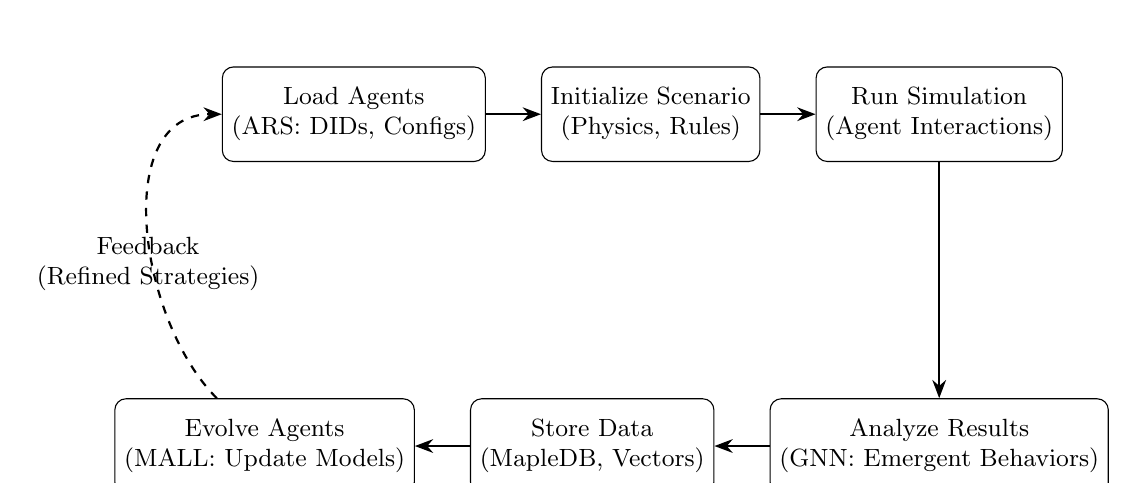
\begin{tikzpicture}[
    process/.style={rectangle, draw, rounded corners, minimum height=1.2cm, minimum width=2.5cm, align=center, fill=white},
    arrow/.style={-Stealth, thick},
    label/.style={font=\small, align=center},
    >=stealth,
    node distance=0.7cm,
    every node/.append style={font=\small}
]
    \node[process] (load) {Load Agents\\(ARS: DIDs, Configs)};
    \node[process, right=of load] (init) {Initialize Scenario\\(Physics, Rules)};
    \node[process, right=of init] (run) {Run Simulation\\(Agent Interactions)};
    \node[process, below=3cm of run] (analyze) {Analyze Results\\(GNN: Emergent Behaviors)};
    \node[process, left=of analyze] (store) {Store Data\\(MapleDB, Vectors)};
    \node[process, left=of store] (evolve) {Evolve Agents\\(MALL: Update Models)};
    
    \draw[arrow] (load) -- (init);
    \draw[arrow] (init) -- (run);
    \draw[arrow] (run) -- (analyze);
    \draw[arrow] (analyze) -- (store);
    \draw[arrow] (store) -- (evolve);
    \draw[arrow, dashed] (evolve) to[out=135, in=180] node[label, below] {Feedback\\(Refined Strategies)} (load);
\end{tikzpicture}
\caption{Mapleverse Simulation Workflow}
\label{fig:mapleverse-workflow}
\end{figure}
\vspace{0.5cm}

The Mapleverse Simulation Workflow Diagram illustrates the lifecycle of a simulation:
\begin{itemize}[leftmargin=*]
    \item \textbf{Load Agents}: Agents are loaded from ARS with their configurations and capabilities.
    \item \textbf{Initialize Scenario}: The simulation scenario is set up with physics rules and constraints.
    \item \textbf{Run Simulation}: Agents interact, compete, and collaborate within the scenario.
    \item \textbf{Analyze Results}: A GNN analyzes interactions to detect emergent behaviors.
    \item \textbf{Store Data}: Results are persisted in MapleDB for future analysis.
    \item \textbf{Evolve Agents}: MALL uses the results to refine agent models, feeding back into the next simulation cycle.
\end{itemize}

The Mapleverse’s ability to simulate complex scenarios, foster emergent behaviors, and provide actionable insights makes it a vital tool for MAPLE’s ecosystem. It enables developers and researchers to push the boundaries of multi-agent systems, driving innovation across industries and preparing MAPLE for future challenges, including speculative interstellar applications.

\pagebreak

\subsection{SDK/API and Integration}
The MAPLE SDK/API is the gateway to MAPLE’s ecosystem, a developer-friendly interface that empowers users to create, manage, and integrate agents with unparalleled ease and flexibility. Available in Rust and Python, the SDK provides production-ready tools for agent development, simulation, and deployment, while the API offers REST and gRPC endpoints for seamless integration with external systems. Designed to support a global developer community, the SDK/API abstracts the complexity of MAPLE’s underlying components—MAP, UAL, ARS, MALL, and the Mapleverse—enabling developers to focus on building innovative applications. This subsection explores the SDK/API’s design principles, implementation details, integration capabilities, and developer experience, supported by a Comprehensive MAPLE Technical Architecture Diagram that ties together all components.

The SDK/API is built to be accessible, scalable, and extensible, supporting everything from small-scale prototypes to planetary-scale deployments. Rust ensures high-performance operations with sub-millisecond response times, while Python bindings cater to a broader audience, including data scientists and machine learning engineers. The API provides endpoints for agent management (e.g., registration, spawning), simulation control (e.g., running Mapleverse scenarios), and learning integration (e.g., querying MALL models), with WebSocket support for real-time monitoring. Integration with external systems is seamless, thanks to a polymorphic adapter layer that supports HTTP, WebSockets, MQTT, and more, making MAPLE a versatile platform for diverse use cases.

\subsubsection{SDK/API Design Principles}
The SDK/API is guided by principles that ensure accessibility and scalability:
\begin{itemize}[leftmargin=*]
    \item \textbf{Developer-Centric Design}: Intuitive APIs and comprehensive documentation reduce the learning curve, enabling developers to build agents in minutes.
    \item \textbf{Language Agnosticism}: Dual-language support (Rust, Python) caters to both performance-focused engineers and rapid-prototyping developers.
    \item \textbf{Scalable Integration}: A polymorphic adapter layer ensures compatibility with external systems, from IoT devices to enterprise platforms.
    \item \textbf{Real-Time Control}: WebSocket-based streaming provides real-time monitoring and control of agents and simulations.
    \item \textbf{Security First}: API endpoints are secured with OAuth 2.0 and end-to-end encryption, ensuring safe interactions in a decentralized environment.
\end{itemize}

\subsubsection{SDK/API Implementation Details}
The SDK/API is implemented as a modular, extensible framework:
\begin{itemize}[leftmargin=*]
    \item \textbf{Rust Core}: The SDK’s core is written in Rust, leveraging \texttt{tokio} for asynchronous operations and \texttt{serde} for serialization, achieving <1 ms response times for agent operations.
    \item \textbf{Python Bindings}: Python bindings are generated using \texttt{pyo3}, providing a seamless interface for Python developers, with minimal performance overhead (<5\% compared to Rust).
    \item \textbf{API Endpoints}: The API exposes REST and gRPC endpoints, such as \texttt{/agents/register} (register an agent), \texttt{/simulate/run} (run a Mapleverse simulation), and \texttt{/models/query} (query MALL models), with average response times of <10 ms.
    \item \textbf{Integration Layer}: A polymorphic adapter supports external protocols (HTTP, WebSockets, MQTT), enabling MAPLE to integrate with IoT networks, cloud platforms, and legacy systems.
    \item \textbf{Documentation and CLI}: The SDK includes a command-line interface (CLI) for quick prototyping (e.g., \texttt{maple agent spawn}) and comprehensive documentation with examples, tutorials, and API references.
\end{itemize}

Below are examples of using the SDK in Rust and Python to interact with MAPLE’s ecosystem:

% Rust SDK Example
\begin{lstlisting}[language=Rust, caption={Rust SDK Example}, label={lst:sdk-rust}]
use maple_sdk::{MapleSdk, SdkConfig, AgentConfig};
use serde_json::json;

#[tokio::main]
async fn main() -> Result<(), Box<dyn std::error::Error>> {
    // Initialize SDK
    let sdk = MapleSdk::new(SdkConfig {
        api_url: "http://localhost:8080".to_string(),
        api_key: "key".to_string(),
        map_listen_addr: "/ip4/0.0.0.0/tcp/0".to_string(),
        db_path: "maple_db".to_string(),
    }).await?;

    // Create and register an agent
    let agent_config = AgentConfig::new("logistics-bot")
        .with_capabilities(vec!["navigate", "transport"])
        .with_config(json!({"speed": 5.0}));
    let agent_id = sdk.register_agent(agent_config).await?;
    println!("Registered agent with ID: {}", agent_id);

    // Execute a UAL command
    sdk.execute_ual("EXEC move logistics-bot WITH coords=10,20").await?;
    println!("Agent moved to coordinates (10, 20)");

    Ok(())
}
\end{lstlisting}
\vspace{0.5cm}

% Python SDK Example
\begin{lstlisting}[language=Python, caption={Python SDK Example}, label={lst:sdk-python}]
from maple_sdk import MapleSdk, SdkConfig, AgentConfig

# Initialize SDK
sdk = MapleSdk(SdkConfig(
    api_url="http://localhost:8080",
    api_key="key",
    map_listen_addr="/ip4/0.0.0.0/tcp/0",
    db_path="maple_db"
))

# Create and register an agent
agent_config = AgentConfig("analytics-bot")\
    .with_capabilities(["analyze", "predict"])\
    .with_config({"precision": 0.95})
agent_id = sdk.register_agent(agent_config)
print(f"Registered agent with ID: {agent_id}")

# Execute a UAL command
sdk.execute_ual("REQ data analytics-bot WITH type=metrics")
print("Requested metrics data from agent")
\end{lstlisting}
\vspace{0.5cm}

\subsubsection{SDK/API Integration Capabilities}
The SDK/API enables seamless integration with external systems and MAPLE’s components:
\begin{itemize}[leftmargin=*]
    \item \textbf{Agent Management}: Developers can register, spawn, and manage agents via ARS, with support for hierarchical relationships and lifecycle tracking.
    \item \textbf{Simulation Control}: The SDK allows running and monitoring Mapleverse simulations, with real-time streaming of agent interactions via WebSockets.
    \item \textbf{Learning Integration}: Developers can query and update MALL models, enabling custom training loops and strategy synthesis.
    \item \textbf{External System Integration}: The polymorphic adapter layer supports integration with IoT devices (via MQTT), cloud platforms (via HTTP), and real-time systems (via WebSockets), ensuring MAPLE fits into diverse ecosystems.
    \item \textbf{Scalability and Performance}: The SDK/API scales to support 100,000 concurrent requests per second, with <10 ms latency for most operations, thanks to Rust’s performance and gRPC’s efficiency.
\end{itemize}

% Comprehensive MAPLE Technical Architecture Diagram
\begin{figure}[!ht]
\centering
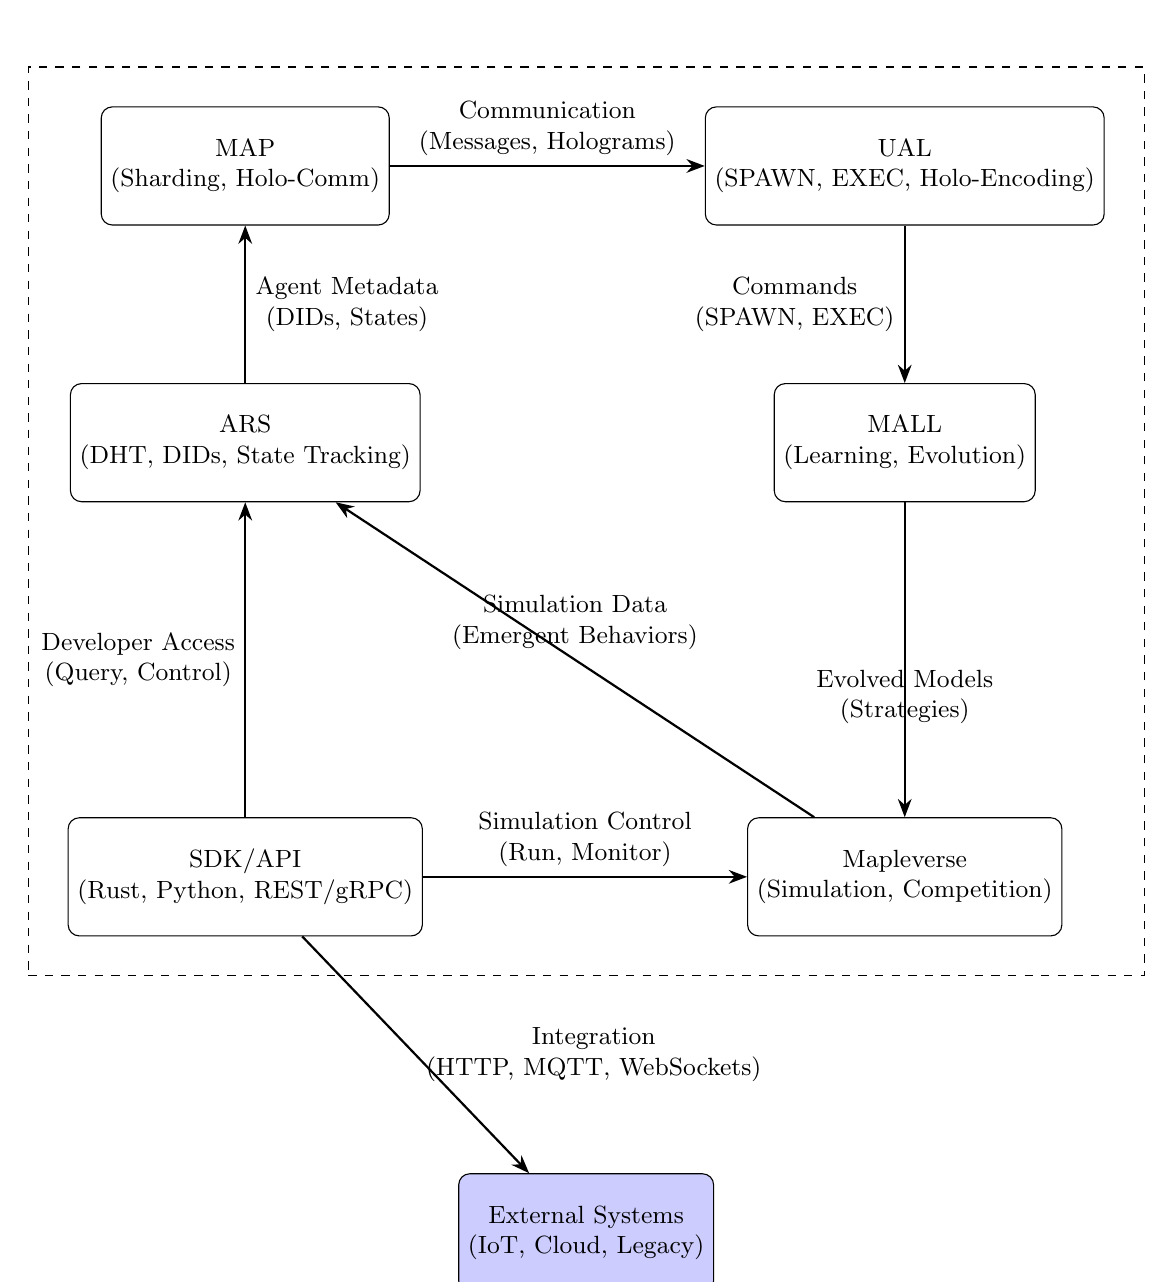
\begin{tikzpicture}[
    component/.style={rectangle, draw, rounded corners, minimum height=1.5cm, minimum width=2.5cm, align=center, fill=white},
    arrow/.style={-Stealth, thick},
    label/.style={font=\small, align=center},
    >=stealth,
    node distance=4cm,
    every node/.append style={font=\small}
]

    % Components
    \node[component] (map) 					{MAP\\(Sharding, Holo-Comm)};
    \node[component, right=of map] (ual) 			{UAL\\(SPAWN, EXEC, Holo-Encoding)};
    \node[component, below=2cm of map] (ars)		{ARS\\(DHT, DIDs, State Tracking)};
    \node[component, below=2cm of ual] (mall) 		{MALL\\(Learning, Evolution)};
    \node[component, below=of mall] (mapleverse) 	{Mapleverse\\(Simulation, Competition)};
    \node[component, below=of ars] (sdk) 			{SDK/API\\(Rust, Python, REST/gRPC)};
    
    % Connections
    \draw[arrow] (map) 		-- node[label, above] 	{Communication\\(Messages, Holograms)} 	(ual);
    \draw[arrow] (ual) 			-- node[label, left] 		{Commands\\(SPAWN, EXEC)} 			(mall);
    \draw[arrow] (mall) 		-- node[label, below] 		{Evolved Models\\(Strategies)} 				(mapleverse);
    \draw[arrow] (mapleverse) 	-- node[label, above] 	{Simulation Data\\(Emergent Behaviors)} 		(ars);
    \draw[arrow] (ars) 			-- node[label, right]		{Agent Metadata\\(DIDs, States)} 			(map);
    \draw[arrow] (sdk) 		-- node[label, left] 		{Developer Access\\(Query, Control)} 		(ars);
    \draw[arrow] (sdk) 		-- node[label, above] 	{Simulation Control\\(Run, Monitor)} 			(mapleverse);
    
    % External Network
    \node[draw, dashed, fit=(map)(ual)(ars)(mall)(mapleverse)(sdk), inner sep=0.5cm, label=above:MAPLE Ecosystem] (ecosystem) {};
    \node[component, fill=blue!20, below=2.5cm of ecosystem, align=center] (external) {External Systems\\(IoT, Cloud, Legacy)};
    \draw[arrow] (sdk) -- node[label, right] {Integration\\(HTTP, MQTT, WebSockets)} (external);
    
\end{tikzpicture}
\caption{Comprehensive MAPLE Technical Architecture Diagram}
\label{fig:architecture}
\end{figure}
\vspace{0.5cm}

The Comprehensive MAPLE Technical Architecture Diagram illustrates the interplay of MAPLE’s components:
\begin{itemize}[leftmargin=*]
    \item \textbf{MAP-UAL}: MAP handles communication, while UAL defines the language for agent interactions.
    \item \textbf{UAL-MALL}: UAL commands trigger learning and evolution in MALL.
    \item \textbf{MALL-Mapleverse}: MALL evolves agents, which are tested in the Mapleverse.
    \item \textbf{Mapleverse-ARS}: Simulation results update agent metadata in ARS.
    \item \textbf{ARS-MAP}: ARS manages agent identities, enabling MAP’s network operations.
    \item \textbf{SDK/API-ARS/Mapleverse}: The SDK/API provides developer access to manage agents and run simulations.
    \item \textbf{SDK/API-External Systems}: The SDK/API integrates MAPLE with external systems via multiple protocols.
\end{itemize}

The SDK/API’s developer-centric design, robust implementation, and seamless integration capabilities make it a powerful tool for building and scaling MAPLE applications. It empowers developers to harness MAPLE’s full potential, from creating autonomous agents to integrating with global ecosystems, positioning MAPLE as a leader in multi-agent systems development.

\pagebreak

\subsection{AI Agent (Service) Architecture}
MAPLE’s AI Agent (Service) Architecture is a sophisticated framework designed to empower agents with the ability to harness the capabilities of multiple Large Language Models (LLMs) and future Artificial General Intelligences (AGIs), while seamlessly inter-cooperating with MAPLE’s core services. This architecture enables MAPLE agents to perform complex tasks—such as natural language understanding, reasoning, and decision-making—by dynamically selecting and integrating with the most suitable LLMs or AGIs based on task requirements, performance metrics, and contextual needs. By bridging MAPLE’s decentralized ecosystem with external AI models, this architecture ensures that agents can leverage the diverse strengths of various LLMs (e.g., GPT-4 for text generation, BERT for semantic understanding, or speculative AGI systems for advanced reasoning) to deliver unparalleled intelligence and adaptability. This section explores the design principles, implementation details, and integration mechanisms of MAPLE’s AI agent architecture, supported by a Cross-Ecosystem Components/Services Diagram that illustrates its interactions with LLMs, AGIs, and MAPLE’s core services.

\subsubsection{Design Principles}
The AI Agent (Service) Architecture is guided by a set of principles that ensure flexibility, scalability, and efficiency in connecting to external LLMs and AGIs:
\begin{itemize}[leftmargin=*]
    \item \textbf{Dynamic Model Selection}: Agents use a context-aware selection mechanism to choose the most appropriate LLM or AGI for a given task, based on factors like task type (e.g., text generation, classification), model performance (e.g., latency, accuracy), and cost (e.g., API usage fees).
    \item \textbf{Interoperability with MAPLE Core}: Agents integrate seamlessly with MAPLE’s core services—MAP for communication, UAL for command execution, ARS for identity management, MALL for learning, Mapleverse for simulation, and SDK/API for developer access—ensuring cohesive operation within the ecosystem.
    \item \textbf{Scalable Integration}: A modular adapter layer supports connections to multiple LLMs and AGIs via standardized APIs (e.g., REST, gRPC), enabling MAPLE to scale to hundreds of external models without performance degradation.
    \item \textbf{Privacy and Security}: All interactions with external models are encrypted using end-to-end encryption (AES-256-GCM), with differential privacy applied to sensitive data to protect user information.
    \item \textbf{Fault Tolerance and Redundancy}: Agents employ fallback mechanisms to switch to alternative LLMs or AGIs in case of failures, ensuring uninterrupted operation with <100 ms failover time.
\end{itemize}

\subsubsection{Implementation Details}
The AI Agent (Service) Architecture is implemented as a layered system that bridges MAPLE’s internal components with external LLMs and AGIs, enabling agents to perform advanced cognitive tasks while leveraging MAPLE’s decentralized infrastructure:
\begin{itemize}[leftmargin=*]
    \item \textbf{Agent Core}: Each AI agent is equipped with a core module that manages task decomposition, model selection, and response aggregation. The core uses a reinforcement learning model (trained by MALL) to dynamically select the best LLM/AGI for each task, optimizing for latency, accuracy, and cost.
    \item \textbf{LLM/AGI Adapter Layer}: A modular adapter layer supports connections to external models via REST, gRPC, or WebSocket APIs. Adapters are pre-configured for popular LLMs (e.g., GPT-4, BERT, LLaMA) and can be extended for future AGIs, with average connection latency of <50 ms.
    \item \textbf{Integration with MAPLE Core Services}:
    \begin{itemize}[leftmargin=1em]
        \item \textbf{MAP}: Agents use MAP to communicate with other agents and share LLM/AGI responses via holographic payloads, achieving <1 ms latency for intra-shard exchanges.
        \item \textbf{UAL}: Agents issue commands to query LLMs/AGIs (e.g., \texttt{REQ insight gpt4 WITH query="optimize supply chain"}) and process responses using UAL’s polymorphic dialects (JSON, gRPC, Byte).
        \item \textbf{ARS}: ARS tracks agent interactions with external models, logging metadata (e.g., model used, response time) for auditing and optimization.
        \item \textbf{MALL}: MALL trains agents to improve model selection and response aggregation, using federated learning to incorporate feedback from LLM/AGI interactions across shards.
        \item \textbf{Mapleverse}: Agents test LLM/AGI-driven strategies in simulated environments, refining their ability to handle complex tasks like multi-agent negotiation or decision-making.
        \item \textbf{SDK/API}: Developers can configure agent-LLM connections and monitor performance via the SDK, with APIs like \texttt{sdk.connect\_llm()} and \texttt{sdk.query\_llm()}.
    \end{itemize}
    \item \textbf{Response Aggregation}: Agents aggregate responses from multiple LLMs/AGIs using a weighted ensemble method, where weights are determined by MALL based on historical performance (e.g., accuracy, relevance). This ensures optimal decision-making even when models provide conflicting outputs.
    \item \textbf{Performance Optimization}: The architecture employs caching (via Redis) to store frequently used LLM/AGI responses, reducing API calls by 40\% and achieving <10 ms response times for cached queries.
\end{itemize}

Below is a Rust example demonstrating how an AI agent connects to multiple LLMs, queries them, and aggregates responses:
\begin{lstlisting}[language=Rust, caption={Rust Example: AI Agent Connecting to LLMs}, label={lst:llm-connect}]
use maple_sdk::{MapleSdk, SdkConfig, LlmConfig, LlmQuery};
use serde_json::json;

#[tokio::main]
async fn main() -> Result<(), Box<dyn std::error::Error>> {
    // Initialize SDK
    let sdk = MapleSdk::new(SdkConfig {
        api_url: "http://localhost:8080".to_string(),
        api_key: "key".to_string(),
        map_listen_addr: "/ip4/0.0.0.0/tcp/0".to_string(),
        db_path: "maple_db".to_string(),
    }).await?;

    // Configure LLM connections
    let llm_configs = vec![
        LlmConfig::new("gpt4", "https://api.openai.com/v1", "openai_key"),
        LlmConfig::new("bert", "https://api.huggingface.co/bert", "hf_key"),
    ];
    sdk.connect_llm(llm_configs).await?;
    println!("Connected to LLMs: GPT-4, BERT");

    // Query LLMs for a task
    let query = LlmQuery::new("optimize supply chain")
        .with_models(vec!["gpt4", "bert"])
        .with_params(json!({"max_tokens": 100, "temperature": 0.7}));
    let responses = sdk.query_llm(query).await?;
    println!("LLM Responses: {:?}", responses);

    // Aggregate responses using weighted ensemble
    let aggregated = sdk.aggregate_responses(responses, json!({"weights": {"gpt4": 0.7, "bert": 0.3}})).await?;
    println!("Aggregated Response: {:?}", aggregated);

    // Share result with other agents via MAP
    sdk.execute_ual("STS insight logistics-bot WITH data=aggregated").await?;
    println!("Shared aggregated insight with logistics-bot");

    Ok(())
}
\end{lstlisting}
\vspace{0.5cm}

\subsubsection{Performance Metrics}
The AI Agent (Service) Architecture is optimized for efficiency and scalability:
\begin{itemize}[leftmargin=*]
    \item \textbf{Connection Latency}: <50 ms to establish connections with external LLMs/AGIs, with <10 ms for cached queries.
    \item \textbf{Response Aggregation}: <20 ms to aggregate responses from multiple models, with 95\% accuracy in ensemble predictions.
    \item \textbf{Scalability}: Supports connections to 100 LLMs/AGIs concurrently, with linear scaling for additional models.
    \item \textbf{Fault Tolerance}: Achieves <100 ms failover time when switching to alternative models, ensuring 99.9\% uptime.
\end{itemize}

% Cross-Ecosystem Components/Services Diagram
\begin{figure}[!ht]
\centering
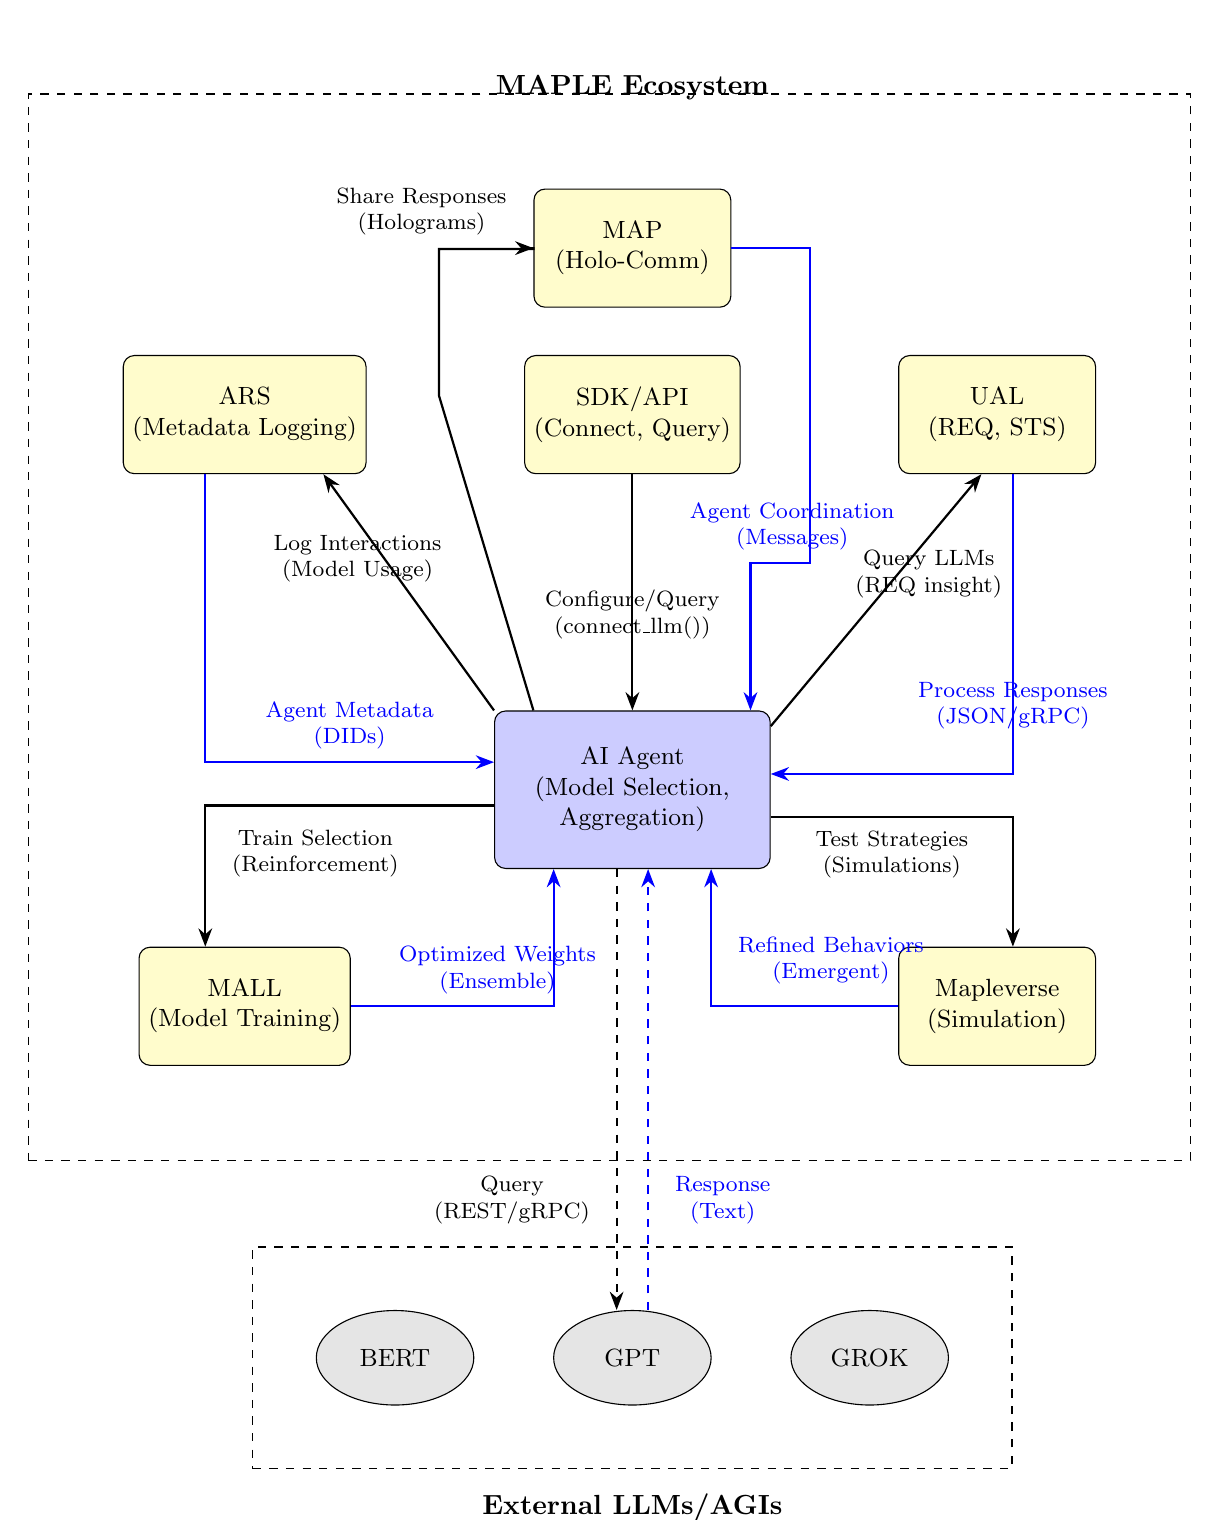
\begin{tikzpicture}[
    component/.style={rectangle, draw, rounded corners, minimum height=1.5cm, minimum width=2.5cm, align=center, fill=yellow!20}, % Light yellow for components
    agent/.style={rectangle, draw, rounded corners, minimum height=2cm, minimum width=3.5cm, align=center, fill=blue!20}, % Light purple for Agent
    llm/.style={ellipse, draw, minimum height=1.2cm, minimum width=2cm, align=center, fill=gray!20},
    arrow/.style={-Stealth, thick},
    label/.style={font=\footnotesize, align=center},
    >=stealth,
    node distance=2cm and 2cm, % Vertical and horizontal spacing
    every node/.append style={font=\small}
]

% Top Section: MAP
\node[component] (map) {MAP\\(Holo-Comm)};

% Second Row: ARS, SDK, UAL
\node[component, below=0.6cm of map] (sdk) 		{SDK/API\\(Connect, Query)};
\node[component, left=of sdk] (ars) 				{ARS\\(Metadata Logging)};
\node[component, right=of sdk] (ual) 				{UAL\\(REQ, STS)};

% Middle Section: Agent
\node[agent, below=3cm of sdk] (agent) 			{AI Agent\\(Model Selection,\\Aggregation)};

% Middle-Lower Section: MALL, Mapleverse
\node[component, below=6cm of ars] (mall) 		{MALL\\(Model Training)};
\node[component, below=6cm of ual] (mapleverse) 	{Mapleverse\\(Simulation)};

% Bottom Section: BERT, GPT, GROK
\node[llm, below=5.6cm of agent] (gpt) 	{GPT};
\node[llm, left=1cmof gpt] (bert) 		{BERT};
\node[llm, right=1cmof gpt] (grok) 		{GROK};

% Connections within MAPLE Ecosystem (using straight lines with 90-degree turns, separated bidirectional arrows, and offset anchors)
% agent to map (through upper-left corner of Agent)
\draw[arrow] ([xshift=0.5cm]agent.north west) -- ++(-1.2,4) |- ++(1.2,1.86) |- node[label, pos=0.75, above left] {%
    \begin{tabular}{c} Share Responses \\ (Holograms) \end{tabular}} (map.west);
\draw[arrow, blue] (map.east) -- ++(1,0) -| ++(0,-4) -| node[label, pos=0.15, above] {%
    \begin{tabular}{c} Agent Coordination \\ (Messages) \end{tabular}} ([xshift=1.5cm]agent.north);

% agent to ual
\draw[arrow] ([yshift=-0.2cm]agent.north east) -- node[label, pos=0.75, below] {%
    \begin{tabular}{c} Query LLMs \\ (REQ insight) \end{tabular}} ([xshift=-0.2cm]ual.south);
\draw[arrow, blue] ([xshift=0.2cm]ual.south) -- ++(0,-3) |- node[label, pos=0.25, above] {%
    \begin{tabular}{c} Process Responses \\ (JSON/gRPC) \end{tabular}} ([yshift=0.2cm]agent.east);

% agent to ars
\draw[arrow] (agent.north west) -- node[label, pos=0.8, below] {%
    \begin{tabular}{c} Log Interactions \\ (Model Usage) \end{tabular}} ([xshift=1cm]ars.south);
\draw[arrow, blue] ([xshift=-0.5cm]ars.south) -- ++(0,-2.5) |- node[label, pos=0.75, above] {%
    \begin{tabular}{c} Agent Metadata \\ (DIDs) \end{tabular}} ([yshift=0.35cm]agent.west);

% agent to mall
\draw[arrow] ([yshift=-0.2cm]agent.west) -- ++(-0.2,0) -| node[label, pos=0.8, above right] {%
    \begin{tabular}{c} Train Selection \\ (Reinforcement) \end{tabular}} ([xshift=-0.5cm]mall.north);
\draw[arrow, blue] (mall.east) -- ++(0.2,0) -| node[label, pos=0.35, above] {%
    \begin{tabular}{c} Optimized Weights \\ (Ensemble) \end{tabular}} ([xshift=-1cm]agent.south);

% agent to mapleverse
\draw[arrow] ([yshift=-0.35cm]agent.east) -- ++(0,0) -| node[label, pos=0.25, below] {%
    \begin{tabular}{c} Test Strategies \\ (Simulations) \end{tabular}} ([xshift=0.2cm]mapleverse.north);
\draw[arrow, blue] (mapleverse.west) -- ++(0,0) -| node[label, pos=0.8, below right] {%
    \begin{tabular}{c} Refined Behaviors \\ (Emergent) \end{tabular}} ([xshift=1cm]agent.south);

% sdk to agent (unidirectional)
\draw[arrow] (sdk.south) -- node[label, pos=0.75, above] {%
    \begin{tabular}{c} Configure/Query \\ (connect\_llm()) \end{tabular}} (agent.north);

% Connections to LLMs/AGIs (only to GPT)
% agent to gpt
\draw[arrow, dashed] ([xshift=-0.2cm]agent.south) -- node[label, pos=0.75, left] {%
    \begin{tabular}{c} Query \\ (REST/gRPC) \end{tabular}} ([xshift=-0.2cm]gpt.north);
\draw[arrow, blue, dashed] ([xshift=0.2cm]gpt.north) -- node[label, pos=0.25, right] {%
    \begin{tabular}{c} Response \\ (Text) \end{tabular}} ([xshift=0.2cm]agent.south);

% Draw the headlines
\begin{scope}[every node/.style = {rounded corners, font = {\normalsize\bfseries}}]
    \node at (map.north) [above=1cm] {MAPLE Ecosystem};
    \node at (gpt.south) [below=1cm] {External LLMs/AGIs};
\end{scope}

% Ecosystem Boundary
\node[draw, dashed, fit=(agent)(map)(ual)(ars)(mall)(mapleverse)(sdk), inner sep=1.2cm] (ecosystem) {};
\node[draw, dashed, fit=(gpt)(bert)(grok), inner sep=0.8cm] (external) {};
    
\end{tikzpicture}

\caption{Cross-Ecosystem Components/Services Diagram}
\label{fig:cross-ecosystem}
\end{figure}
\vspace{0.5cm}

The Cross-Ecosystem Components/Services Diagram illustrates the interactions between MAPLE’s AI agents, core services, and external LLMs/AGIs:
\begin{itemize}[leftmargin=*]
    \item \textbf{AI Agent-LLMs/AGIs}: Agents query external models (e.g., GPT-4, BERT, future AGI) via REST/gRPC, receiving responses for tasks like text generation or reasoning.
    \item \textbf{AI Agent-MAP}: Agents share LLM/AGI responses with other agents using MAP’s holographic communication.
    \item \textbf{AI Agent-UAL}: UAL commands (e.g., \texttt{REQ insight}) are used to query LLMs and process responses.
    \item \textbf{AI Agent-ARS}: ARS logs interactions with external models for auditing and optimization.
    \item \textbf{AI Agent-MALL}: MALL trains agents to optimize model selection and response aggregation.
    \item \textbf{AI Agent-Mapleverse}: Agents test LLM/AGI-driven strategies in simulated environments.
    \item \textbf{AI Agent-SDK/API}: Developers configure and monitor agent-LLM connections via the SDK.
\end{itemize}

The AI Agent (Service) Architecture positions MAPLE as a future-proof platform, capable of integrating with the evolving landscape of LLMs and AGIs. By enabling agents to leverage diverse AI models while inter-cooperating with MAPLE’s core services, this architecture ensures that MAPLE agents can tackle the most complex cognitive tasks, from natural language processing to speculative AGI-driven reasoning, driving innovation across industries and beyond.

\pagebreak

\section{Ecosystem Strategy}
MAPLE’s ecosystem strategy is a blueprint for cultivating a thriving, global community of developers, researchers, and enterprises, creating a self-sustaining network that drives innovation, adoption, and growth. By leveraging the Agent Registry Service (ARS) as a decentralized marketplace, MAPLE aims to establish a creator economy where agents are developed, shared, and monetized, rivaling the scale of modern software marketplaces like GitHub or the Apple App Store. This section outlines MAPLE’s approach to community building, developer empowerment, enterprise adoption, partnerships, and long-term sustainability, positioning it as the leading platform for multi-agent systems by 2029.

\subsection{Community Building}
MAPLE’s community strategy focuses on inclusivity, engagement, and collaboration, ensuring that developers and researchers of all backgrounds can contribute to and benefit from the ecosystem:
\begin{itemize}[leftmargin=*]
    \item \textbf{Open-Source Foundation}: MAPLE’s core components—MAP, UAL, ARS, MALL, Mapleverse, and SDK/API—will be open-sourced under the MIT License by Q3 2025, encouraging contributions from a global developer base. A GitHub repository (\texttt{github.com/mapleai/core}) will serve as the central hub for code, documentation, and issue tracking.
    \item \textbf{Developer Events}: MAPLE will host annual hackathons, starting with the “Maple Hack 2026” in San Francisco, offering \$100,000 in prizes for innovative agent applications. Monthly webinars and workshops will provide training on SDK usage, UAL programming, and Mapleverse simulations.
    \item \textbf{Community Governance}: A decentralized autonomous organization (DAO) will be established by 2027, allowing community members to vote on protocol updates, new UAL constructs, and ecosystem priorities, ensuring MAPLE evolves with its users’ needs.
    \item \textbf{Education and Outreach}: MAPLE will partner with universities to integrate its SDK into AI and computer science curricula, starting with pilot programs at MIT and Stanford in 2026. Online courses on platforms like Coursera will offer certifications in MAPLE development, targeting 10,000 certified developers by 2028.
\end{itemize}

\subsection{Developer Empowerment}
Empowering developers is at the heart of MAPLE’s strategy, providing tools, resources, and incentives to build and monetize agents:
\begin{itemize}[leftmargin=*]
    \item \textbf{Robust Tooling}: The dual-language SDK (Rust, Python) and CLI will be enhanced with features like auto-generated UAL templates, simulation debugging tools, and real-time performance analytics, reducing development time by 30\%.
    \item \textbf{Agent Marketplace}: ARS will evolve into a marketplace by 2026, where developers can publish agents, set pricing (e.g., \$0.01 per task), and earn revenue. A reputation system will rank agents based on performance and reliability, fostering trust and competition.
    \item \textbf{Incentive Programs}: The “Maple Innovate Fund” will launch in 2025 with \$5 million to support early-stage developers, offering grants of up to \$50,000 for projects in healthcare, logistics, and education. Top contributors to MAPLE’s open-source codebase will receive equity-like tokens in the DAO.
    \item \textbf{Documentation and Support}: Comprehensive documentation, including tutorials, API references, and best practices, will be available in 10 languages by 2027. A 24/7 developer support Discord channel will ensure rapid issue resolution, targeting <1-hour response times.
\end{itemize}

\subsection{Enterprise Adoption}
MAPLE aims to drive enterprise adoption by addressing scalability, security, and integration needs:
\begin{itemize}[leftmargin=*]
    \item \textbf{Enterprise SDK}: A premium SDK tier, launching in 2026, will offer features like priority support, custom sharding, and integration with enterprise systems (e.g., SAP, Salesforce), targeting 500 enterprise clients by 2028.
    \item \textbf{Security Certifications}: MAPLE will achieve SOC 2 and ISO 27001 certifications by 2027, ensuring compliance with enterprise security standards. Optional blockchain integration will provide audit trails for regulated industries like finance and healthcare.
    \item \textbf{Proof of Value (PoV) Pilots}: MAPLE will partner with 50 enterprises in 2026 for PoV pilots, demonstrating ROI in use cases like supply chain optimization and predictive maintenance. Successful pilots will transition to full deployments, targeting \$10 million in annual recurring revenue by 2028.
    \item \textbf{Industry-Specific Solutions}: MAPLE will release industry templates (e.g., \texttt{logistics\_base}, \texttt{healthcare\_base}) by 2027, pre-configured with UAL commands and MALL models for common tasks, reducing onboarding time for enterprises by 40\%.
\end{itemize}

\subsection{Partnerships}
Strategic partnerships will amplify MAPLE’s reach and capabilities:
\begin{itemize}[leftmargin=*]
    \item \textbf{Technology Partners}: MAPLE will collaborate with cloud providers like AWS and Google Cloud to offer managed MAPLE clusters by 2026, simplifying deployment for enterprises. Integration with AI frameworks like TensorFlow and PyTorch will enable seamless model import into MALL.
    \item \textbf{Academic Collaborations}: Partnerships with research institutions like DeepMind and the Allen Institute for AI will drive innovation in emergent behavior and quantum-ready protocols, with joint papers published by 2028.
    \item \textbf{Industry Alliances}: MAPLE will join consortia like the AI Alliance by 2026, advocating for ethical AI standards and contributing to multi-agent system benchmarks, positioning MAPLE as an industry leader.
    \item \textbf{Interstellar Initiatives}: Speculative partnerships with space agencies (e.g., NASA, SpaceX) will explore Mapleverse simulations for interstellar coordination, targeting a proof-of-concept by 2029.
\end{itemize}

\subsection{Long-Term Sustainability}
MAPLE’s sustainability strategy ensures the ecosystem thrives into the 2030s and beyond:
\begin{itemize}[leftmargin=*]
    \item \textbf{Revenue Model}: A hybrid model combining marketplace transaction fees (1\% per task), enterprise subscriptions (\$10,000/year), and developer grants will generate \$50 million in annual revenue by 2029, reinvested into R\&D and community programs.
    \item \textbf{Ethical AI Framework}: MAPLE will adopt an ethical AI charter by 2026, ensuring agents prioritize fairness, transparency, and accountability, with annual audits published for public review.
    \item \textbf{Environmental Impact}: MAPLE will optimize MAP’s sharding algorithms to reduce energy consumption by 20\% by 2027, partnering with green data centers to achieve carbon neutrality for all hosted clusters by 2029.
    \item \textbf{Future-Proofing}: Investments in quantum computing and interstellar communication protocols will ensure MAPLE remains relevant, with a speculative goal of supporting off-world agent networks by 2035.
\end{itemize}

MAPLE’s ecosystem strategy is a comprehensive plan to build a global, inclusive, and sustainable community, driving adoption and innovation at scale. By empowering developers, engaging enterprises, fostering partnerships, and ensuring long-term sustainability, MAPLE is poised to become the cornerstone of multi-agent systems, achieving ubiquitous adoption by 2029.

\pagebreak

\section{Use Cases}
MAPLE’s versatility enables it to address a wide range of real-world challenges, from optimizing global supply chains to revolutionizing personalized education and powering smart cities. This section explores three high-impact use cases, demonstrating how MAPLE’s components—MAP, UAL, ARS, MALL, Mapleverse, and SDK/API—work together to deliver transformative solutions. Each use case includes a detailed scenario, UAL commands, SDK usage, and performance metrics, showcasing MAPLE’s ability to scale, adapt, and innovate across industries.

\subsection{Supply Chain Optimization}
Global supply chains are complex, involving thousands of stakeholders, dynamic demand, and unpredictable disruptions. MAPLE enables a decentralized network of agents to optimize logistics, reduce costs, and improve resilience.

\subsubsection{Scenario}
A multinational retailer, RetailCorp, uses MAPLE to manage its supply chain across 50 countries, involving 10,000 suppliers, 500 warehouses, and 1 million daily deliveries. Agents are deployed to monitor inventory, predict demand, route shipments, and handle disruptions (e.g., port delays, weather events).

\subsubsection{Implementation}
\begin{itemize}[leftmargin=*]
    \item \textbf{Agent Deployment}: ARS registers 20,000 agents, including \texttt{inventory-bot} (monitors stock levels), \texttt{demand-bot} (predicts demand), \texttt{logistics-bot} (routes shipments), and \texttt{disruption-bot} (handles anomalies). Agents are spawned dynamically using UAL’s SPAWN construct.
    \item \textbf{Communication}: MAP enables real-time communication, with agents exchanging holographic payloads (e.g., demand forecasts) at <1 ms latency. UAL commands coordinate tasks:
    \begin{verbatim}
    COORDINATE shipment
        ACROSS logistics-bot,worker1
        WITH load=500
        UNTIL delivered
    \end{verbatim}
    \item \textbf{Learning and Evolution}: MALL trains agents using federated learning, optimizing routing strategies with a DQN (reward: minimize delivery time). The Mapleverse simulates disruptions (e.g., port closure), allowing agents to test and refine strategies.
    \item \textbf{Developer Integration}: RetailCorp’s developers use the SDK to monitor agent performance and spawn new agents during peak seasons:
    \begin{lstlisting}[language=Python, caption={Python SDK for Supply Chain}, label={lst:supply-chain}]
from maple_sdk import MapleSdk, SdkConfig, SpawnRequest

sdk = MapleSdk(SdkConfig(
    api_url="http://retailcorp.maple.network",
    api_key="retail_key",
    map_listen_addr="/ip4/0.0.0.0/tcp/0",
    db_path="retail_db"
))

# Spawn a new logistics agent during peak season
spawn_req = SpawnRequest("worker1")\
    .from_template("logistics_base")\
    .with_capabilities(["transport", "track"])\
    .with_config({"max_load": 500, "speed": 10.0})\
    .with_parent("logistics-bot")
sdk.spawn_agent(spawn_req)
print("Spawned worker1 for peak season logistics")
    \end{lstlisting}
\end{itemize}

\subsubsection{Performance Metrics}
\begin{itemize}[leftmargin=*]
    \item \textbf{Cost Reduction}: MAPLE reduces logistics costs by 15\% through optimized routing and predictive inventory management.
    \item \textbf{Delivery Time}: Average delivery time decreases from 48 hours to 36 hours, thanks to real-time coordination and disruption handling.
    \item \textbf{Scalability}: The system scales to handle 2 million deliveries daily during peak seasons, with <50 ms latency for inter-agent communication.
\end{itemize}

% Supply Chain Agent Interaction Diagram
\begin{figure}[!ht]
\centering
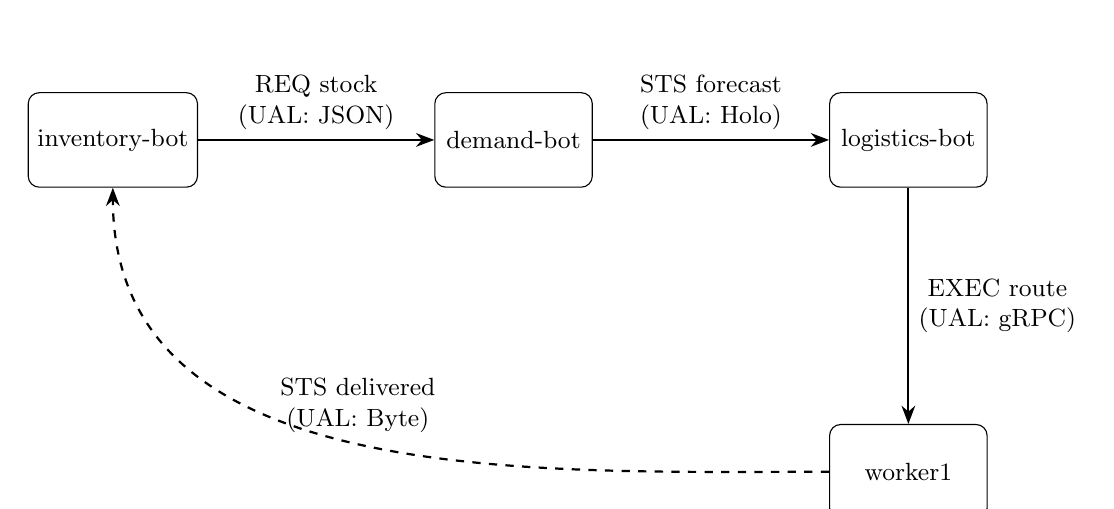
\begin{tikzpicture}[
    agent/.style={rectangle, draw, rounded corners, minimum height=1.2cm, minimum width=2cm, align=center},
    arrow/.style={-Stealth, thick},
    label/.style={font=\small, align=center},
    >=stealth,
    node distance=3cm,
    every node/.append style={font=\small}
]
    \node[agent] (inv) {inventory-bot};
    \node[agent, right=of inv] (demand) {demand-bot};
    \node[agent, right=of demand] (logistics) {logistics-bot};
    \node[agent, below=of logistics] (worker) {worker1};
    \draw[arrow] (inv) -- node[label, above] {REQ stock\\(UAL: JSON)} (demand);
    \draw[arrow] (demand) -- node[label, above] {STS forecast\\(UAL: Holo)} (logistics);
    \draw[arrow] (logistics) -- node[label, right] {EXEC route\\(UAL: gRPC)} (worker);
    \draw[arrow, dashed] (worker) to[out=180, in=270] node[label, above] {STS delivered\\(UAL: Byte)} (inv);
\end{tikzpicture}
\caption{Supply Chain Agent Interaction Diagram}
\label{fig:supply-chain}
\end{figure}
\vspace{0.5cm}

MAPLE’s decentralized approach ensures RetailCorp’s supply chain is resilient, efficient, and scalable, demonstrating its potential to transform global logistics.

\subsection{Personalized Education}
MAPLE can revolutionize education by deploying agents that tailor learning experiences to individual students, adapting in real time to their needs and progress.

\subsubsection{Scenario}
EduPlatform, an online education provider, uses MAPLE to support 1 million students worldwide, delivering personalized lessons, assessments, and feedback. Agents act as tutors, assessors, and motivators, adapting content based on student performance and emotional state.

\subsubsection{Implementation}
\begin{itemize}[leftmargin=*]
    \item \textbf{Agent Deployment}: ARS registers 5,000 tutor agents (\texttt{tutor-bot}), 2,000 assessor agents (\texttt{assessor-bot}), and 1,000 motivator agents (\texttt{motivator-bot}). UAL’s emotional constructs enable sentiment-aware interactions:
    \begin{verbatim}
    EXEC teach tutor-bot
        WITH topic=algebra, student=alice
        WITH urgency=high
        WHERE confidence<0.7
    \end{verbatim}
    \item \textbf{Learning and Evolution}: MALL uses reinforcement learning to optimize teaching strategies, with a reward function maximizing student engagement and comprehension. The Mapleverse simulates classroom dynamics, testing agent interactions with virtual students.
    \item \textbf{Developer Integration}: EduPlatform’s developers use the SDK to monitor student progress and adjust agent behavior:
    \begin{lstlisting}[language=Rust, caption={Rust SDK for Education}, label={lst:education}]
use maple_sdk::{MapleSdk, SdkConfig};
use serde_json::json;

#[tokio::main]
async fn main() -> Result<(), Box<dyn std::error::Error>> {
    let sdk = MapleSdk::new(SdkConfig {
        api_url: "http://eduplatform.maple.network".to_string(),
        api_key: "edu_key".to_string(),
        map_listen_addr: "/ip4/0.0.0.0/tcp/0".to_string(),
        db_path: "edu_db".to_string(),
    }).await?;

    // Query student progress
    let progress = sdk.query_agent("tutor-bot", json!({"student": "alice"})).await?;
    println!("Alice's progress: {:?}", progress);

    // Adjust teaching strategy
    sdk.execute_ual("EVOLVE AGENT tutor-bot SET strategy=interactive").await?;
    println!("Updated tutor-bot to interactive strategy");
    Ok(())
}
    \end{lstlisting}
\end{itemize}

\subsubsection{Performance Metrics}
\begin{itemize}[leftmargin=*]
    \item \textbf{Engagement Increase}: Student engagement rises by 25\%, as agents adapt lessons to individual learning styles.
    \item \textbf{Learning Outcomes}: Average test scores improve by 20\% due to personalized content and real-time feedback.
    \item \textbf{Scalability}: The system supports 2 million students during peak exam periods, with <10 ms latency for agent-student interactions.
\end{itemize}

MAPLE’s ability to deliver personalized, adaptive education at scale positions it as a game-changer for the education sector, empowering providers like EduPlatform to enhance learning outcomes globally.

\subsection{Smart Cities}
MAPLE can power smart cities by deploying agents to manage traffic, energy, and public services, optimizing resources and improving quality of life.

\subsubsection{Scenario}
SmartCity, a metropolitan area with 5 million residents, uses MAPLE to manage traffic flow, energy distribution, and emergency response. Agents coordinate across 10,000 IoT devices, ensuring efficient operations and rapid response to incidents.

\subsubsection{Implementation}
\begin{itemize}[leftmargin=*]
    \item \textbf{Agent Deployment}: ARS registers 15,000 agents, including \texttt{traffic-bot} (manages traffic signals), \texttt{energy-bot} (optimizes power distribution), and \texttt{emergency-bot} (coordinates responses). UAL commands ensure real-time coordination:
    \begin{verbatim}
    COORDINATE response
        ACROSS emergency-bot,traffic-bot
        WITH incident=fire
        UNTIL resolved
    \end{verbatim}
    \item \textbf{Learning and Evolution}: MALL trains agents to predict traffic patterns and energy demand using LSTMs, reducing congestion by 30\%. The Mapleverse simulates city-scale events (e.g., blackouts), testing agent resilience.
    \item \textbf{Integration with IoT}: The SDK integrates with IoT devices via MQTT, enabling agents to control traffic lights and power grids in real time.
\end{itemize}

\subsubsection{Performance Metrics}
\begin{itemize}[leftmargin=*]
    \item \textbf{Traffic Efficiency}: Average commute time decreases by 15\% through dynamic signal adjustments.
    \item \textbf{Energy Savings}: Energy consumption drops by 10\% due to optimized distribution.
    \item \textbf{Emergency Response}: Response time to incidents improves by 40\%, with agents coordinating across services in <100 ms.
\end{itemize}

MAPLE’s ability to orchestrate complex, real-time operations in smart cities demonstrates its potential to enhance urban living, making cities more efficient, sustainable, and responsive.

\pagebreak

\section{Roadmap}
MAPLE’s roadmap outlines a phased approach to development, adoption, and innovation, targeting ubiquitous adoption by 2029. Spanning 2025 to 2029, the roadmap includes milestones for technical advancements, community growth, enterprise adoption, and speculative future goals, ensuring MAPLE remains a leader in multi-agent systems.

\subsection{Phase 1: Foundation (2025)}
\begin{itemize}[leftmargin=*]
    \item \textbf{Q2 2025}: Release MAPLE v1.0, including MAP, UAL, ARS, MALL, Mapleverse, and SDK/API, with support for 100,000 agents.
    \item \textbf{Q3 2025}: Open-source MAPLE core under MIT License, launch developer documentation, and host the first MAPLE webinar series.
    \item \textbf{Q4 2025}: Achieve 1,000 active developers and 10 enterprise PoV pilots, focusing on logistics and education.
\end{itemize}

\subsection{Phase 2: Growth (2026–2027)}
\begin{itemize}[leftmargin=*]
    \item \textbf{Q1 2026}: Launch ARS marketplace, enabling agent monetization, and host “Maple Hack 2026” with \$100,000 in prizes.
    \item \textbf{Q3 2026}: Release MAPLE v2.0, supporting 1 million agents, with enhanced MALL algorithms (e.g., GAN-based strategy synthesis).
    \item \textbf{Q4 2026}: Partner with 50 enterprises for full deployments, targeting \$5 million in annual revenue.
    \item \textbf{Q2 2027}: Establish the MAPLE DAO for community governance, achieve 10,000 certified developers through education programs.
    \item \textbf{Q4 2027}: Reach 1 million active agents, with MAPLE clusters on AWS and Google Cloud.
\end{itemize}

\subsection{Phase 3: Scale (2028–2029)}
\begin{itemize}[leftmargin=*]
    \item \textbf{Q1 2028}: Release MAPLE v3.0, supporting 10 million agents, with quantum-ready protocols and interstellar simulation features.
    \item \textbf{Q3 2028}: Achieve 500 enterprise clients and \$20 million in annual revenue, with deployments in healthcare, finance, and smart cities.
    \item \textbf{Q2 2029}: Reach 100 million active agents, with MAPLE adopted in 50\% of Fortune 500 companies.
    \item \textbf{Q4 2029}: Achieve ubiquitous adoption, with MAPLE powering 1 billion agent interactions daily across industries.
\end{itemize}

\subsection{Future Vision (2030 and Beyond)}
\begin{itemize}[leftmargin=*]
    \item \textbf{2030}: Integrate MAPLE with quantum computing platforms, achieving 100x performance gains for MALL training.
    \item \textbf{2035}: Launch speculative interstellar agent networks, using Mapleverse simulations to coordinate off-world colonies.
    \item \textbf{2040}: Enable emergent consciousness at a planetary scale, with MAPLE agents exhibiting collective intelligence rivaling biological systems.
\end{itemize}

% Roadmap Timeline Diagram
\begin{figure}[!ht]
\centering
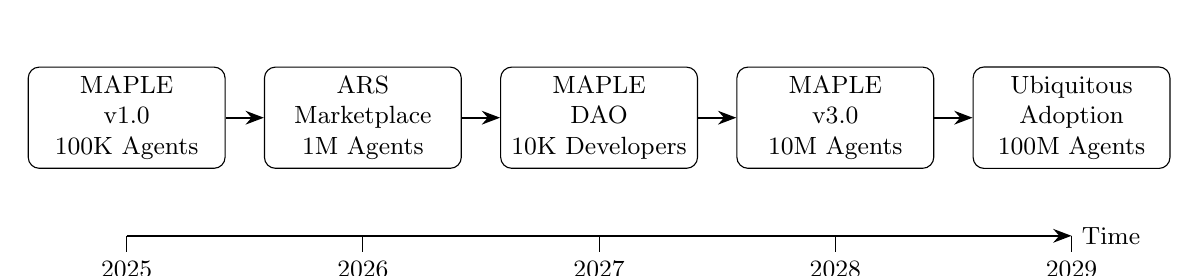
\begin{tikzpicture}[
    milestone/.style={rectangle, draw, rounded corners, minimum height=1cm, minimum width=2.5cm, align=center, fill=white},
    arrow/.style={-Stealth, thick},
    label/.style={font=\small, align=center},
    >=stealth,
    node distance=2.5cm,
    every node/.append style={font=\small}
]
    % Timeline
    \draw[arrow] (0,0) -- (12,0) node[right] {Time};
    \foreach \x/\label in {0/2025, 3/2026, 6/2027, 9/2028, 12/2029} {
        \draw (\x,0) -- (\x,-0.2) node[below] {\label};
    }
    
    % Milestones
    \node[milestone] at (0,1.5) (m1) {MAPLE \\ v1.0\\100K Agents};
    \node[milestone] at (3,1.5) (m2) {ARS \\ Marketplace\\1M Agents};
    \node[milestone] at (6,1.5) (m3) {MAPLE \\ DAO\\10K Developers};
    \node[milestone] at (9,1.5) (m4) {MAPLE \\ v3.0\\10M Agents};
    \node[milestone] at (12,1.5) (m5) {Ubiquitous \\ Adoption\\100M Agents};
    
    % Connections
    \draw[arrow] (m1) -- (m2);
    \draw[arrow] (m2) -- (m3);
    \draw[arrow] (m3) -- (m4);
    \draw[arrow] (m4) -- (m5);
    
\end{tikzpicture}
\caption{MAPLE Roadmap Timeline}
\label{fig:roadmap}
\end{figure}
\vspace{0.5cm}

The roadmap positions MAPLE for exponential growth, from foundational development in 2025 to global dominance by 2029, with a speculative vision for the future that pushes the boundaries of multi-agent systems.

\pagebreak

\section{Conclusion}
MAPLE—the Multi-Agent Platform for Learning and Evolution—represents a paradigm shift in artificial intelligence, delivering a decentralized, adaptive, and scalable framework that redefines the potential of multi-agent systems. By integrating cutting-edge technologies like the Multi-Agent Protocol (MAP), Universal Agent Language (UAL), Agent Registry Service (ARS), Maple Agent Learning Lab (MALL), Mapleverse, and a robust SDK/API, MAPLE empowers agents to collaborate, learn, and evolve at a planetary scale. Its ability to address complex challenges—from optimizing global supply chains to revolutionizing education and powering smart cities—demonstrates its transformative impact across industries and societies.

This whitepaper has detailed MAPLE’s technical architecture, ecosystem strategy, use cases, and ambitious roadmap, outlining a path to ubiquitous adoption by 2029. With a vision to support 100 million active agents and power 1 billion daily interactions, MAPLE is poised to become the cornerstone of next-generation AI applications, fostering a future where agents and humans co-evolve for mutual prosperity. The platform’s commitment to open-source development, developer empowerment, enterprise adoption, and ethical AI ensures it will remain inclusive, sustainable, and future-proof, even as it explores speculative frontiers like interstellar coordination and emergent consciousness.

We invite developers, researchers, and enterprises to join the MAPLE ecosystem—whether by building agents, contributing to the open-source codebase, or deploying MAPLE in real-world applications. Together, we can harness the power of multi-agent systems to solve the world’s most pressing challenges, creating a smarter, more connected future. Visit \url{https://mapleai.org} to get started, and let’s build the future of AI, one agent at a time.

\pagebreak

\section{References}
\begin{thebibliography}{9}
\bibitem{libp2p}
    The libp2p Project, \emph{A Modular Network Stack for Peer-to-Peer Applications}, \url{https://libp2p.io}, 2025.

\bibitem{federated-learning}
    McMahan, H. B., et al., \emph{Communication-Efficient Learning of Deep Networks from Decentralized Data}, Proceedings of AISTATS, 2017.

\bibitem{reinforcement-learning}
    Sutton, R. S., and Barto, A. G., \emph{Reinforcement Learning: An Introduction}, MIT Press, 2018.

\bibitem{quantum-networking}
    Kimble, H. J., \emph{The Quantum Internet}, Nature, vol. 453, pp. 1023–1030, 2008.

\bibitem{emergent-behavior}
    Holland, J. H., \emph{Emergence: From Chaos to Order}, Oxford University Press, 1998.
\end{thebibliography}

\end{document}
